\documentclass[final,3p,times,twocolumn]{elsarticle}
\usepackage[utf8]{inputenc}
\usepackage[T1]{fontenc}
\usepackage[english]{babel}
\usepackage{pifont}
\usepackage{natbib}
\usepackage{geometry}
\usepackage[labelfont=bf]{subcaption}
\usepackage{textcomp}
\usepackage{graphicx}
\usepackage[colorlinks=true,linkcolor=cyan]{hyperref}
\usepackage{amsmath}
\usepackage{amsthm}
\usepackage{amssymb}
\usepackage{amsfonts}
\usepackage{dblfloatfix}
\usepackage{ulem} % package to cross out text

%%%%%%%%%%%%%%%%%%%%%%%
%% Elsevier bibliography styles
%%%%%%%%%%%%%%%%%%%%%%%
%% To change the style, put a % in front of the second line of the current style and
%% remove the % from the second line of the style you would like to use.
%%%%%%%%%%%%%%%%%%%%%%%

\bibliographystyle{model1-num-names}
\usepackage{numcompress}\bibliographystyle{model6-num-names}
\journal{Acta Materiala}

\begin{document}

\begin{frontmatter}

%% Title, authors and addresses

%% use the tnoteref command within \title for footnotes;
%% use the tnotetext command for theassociated footnote;
%% use the fnref command within \author or \address for footnotes;
%% use the fntext command for theassociated footnote;
%% use the corref command within \author for corresponding author footnotes;
%% use the cortext command for theassociated footnote;
%% use the ead command for the email address,
%% and the form \ead[url] for the home page:
%% \title{Title\tnoteref{label1}}
%% \tnotetext[label1]{}
%% \author{Name\corref{cor1}\fnref{label2}}
%% \ead{email address}
%% \ead[url]{home page}
%% \fntext[label2]{}
%% \cortext[cor1]{}
%% \address{Address\fnref{label3}}
%% \fntext[label3]{}

\title{Twin-interface interactions in nanostructured Cu/Ag: molecular dynamics study}
%\tnotetext[t1]{This document is a collaborative effort.}
%\tnotetext[t2]{The second title footnote which is a longer longer than the first one and with an intention to fill in up more than one line while formatting.}

%% use optional labels to link authors explicitly to addresses:
%% \author[label1,label2]{}
%% \address[label1]{}
%% \address[label2]{}

\author[pprime]{R.~Béjaud\corref{cor1}\fnref{fn1}}
\author[pprime]{J.~Durinck}
\author[pprime]{S.~Brochard}

\cortext[cor1]{Corresponding author}
%\cortext[cor2]{Principal corresponding author}
\fntext[fn1]{E-mail address: romuald.bejaud@univ-poitiers.fr (R. Béjaud).}
%\fntext[fn2]{Another author footnote, but a little more


\address[pprime]{Institut Pprime, CNRS - Université de Poitiers - ENSMA, UPR 3346, Département de Physique et Mécanique des Matériaux, Bvd M. et P. Curie, SP2MI, BP 30179, 86962 Futuroscope Chasseneuil Cedex, France}


\begin{abstract}
The interaction of twins with interfaces in nanostructured Cu/Ag is studied using molecular dynamics simulations. The influence of the interface structure on twin nucleation, propagation and thickening is analysed, and the role of the misfit interfacial dislocations mesh is detailed. In particular, we show that the interface can induce, directly or indirectly via Lomer dislocations, the nucleation of twinning dislocations. A thorough description of the involved mechanisms is given. Through this atomic scale approach, our study offers some useful understanding of the mechanical twinning process in nanolamellar composites, where twinning appears to be a common plasticity mechanism.

\end{abstract}

\begin{keyword}

Deformation twins \sep Nanolayered materials \sep Heterophase interfaces \sep Molecular dynamics simulations

%% keywords here, in the form: keyword \sep keyword

%% PACS codes here, in the form: \PACS code \sep code

%% MSC codes here, in the form: \MSC code \sep code
%% or \MSC[2008] code \sep code (2000 is the default)

\end{keyword}

\end{frontmatter}


\section{Introduction}

When they are structured at nanoscale, materials can exhibit properties different from those of the bulk. In particular, in the case of nanolayered or nanotwinned materials, interfaces become predominant over the bulk and govern mechanical properties when the distance between layers or twin boundaries (TBs) decreases. Interfaces can interact in different ways with defects, acting as sources or barriers for dislocations, and lead to a modification of mechanical properties \cite{beyerlein15PMS}. For example, it was shown that nanotwinned materials have improved strength, hardness and ductility \cite{lu04S,lu09S,stukowski10PRB,sansoz07NL}. Several experimental and numerical studies demonstrated that in most cases TBs act as strong barriers for moving dislocations, explaining the increase of the strength in such materials \cite{wu09AM,deng09NL,cao15SM}. Similarly, interesting mechanical properties are encountered in nanolayered materials in which heterophase interfaces were found to be mainly responsible for a strengthening effect \cite{misra01AEM,misra05AM}.

Many of the bimetallic nanolayered composites are usually prepared using techniques like cold rolling, accumulative roll-bonding, and high-pressure torsion  \cite{tian13SM,han12APL}. A high amount of elastic strain is stored in materials during these severe plastic deformation (SPD) processes and is commonly released by mechanical twinning. 
It is well documented that the nucleation of partial dislocations and mechanical twinning is promoted at the nanoscale \cite{chen03S,dehm07AM}. 
This trend is especially true in \textcolor{magenta}{metallic} nanolayered materials.
Indeed, recent experimental studies evidenced that twinning occurs at high stresses or strains in Cu/Nb, Cu/Ag and Cu/Au bimaterials \cite{zheng14AM}.  
It is expected that heterophase interfaces play a crucial role on the onset of mechanical twinning. Depending on the interface type (coherent, semi-coherent or incoherent), twinning dislocations (TDs) may be nucleated from the interface directly in adjacent planes or transmitted from one layer to the other, or may be stopped at the interface leading to a strengthening effect \cite{an15APL}.

Therefore the structure of heterophase interfaces appears to be a key parameter for the plastic mechanisms involved in these particular materials and a fundamental understanding of how interfaces interact with twins becomes essential. Because of the small length and time scales at which the elementary plastic mechanisms occur, atomistic simulations appear to be relevant and efficient tools to study mechanical twinning in nanolayered metals. 

In this study, molecular dynamics simulations were performed to investigate, at the atomic scale, the interaction of twins with interfaces \textcolor{magenta}{in a face centered cubic (FCC) bimetal}, and more precisely the role of misfit dislocations on twin nucleation and thickening. 
%Unlike most of molecular dynamics simulations, 
Our strategy was not to perfectly reproduce experimental situations such as those encountered during SPD processes,
%multilayered systems 
but rather to consider configurations for which twinning is promoted and twin/interface interactions easily analysed. The chosen model is a self-supported thin Cu/Ag film with two commonly experimentally observed interface types, referenced as “heterotwin” and “cube on cube” in the following. Twin/interface interactions are then studied according to the interface type. The simulation model is detailed in section \ref{subpart_model} and a description of both interface types is given in section \ref{subpart_interface}. In section \ref{part_influence}, we first analyse the role of the interface structure on mechanical twinning for a reference case, for a “cube on cube” interface (section \ref{subsubpart_sAg}) and for a “heterotwin” interface (section \ref{subsubpart_sAg2}). Different sites for the first plastic event are then considered in section \ref{subsubpart_comparaison}, in order to assess the sensitivity of the simulation results to this parameter. Finally, in section \ref{part_misfit}, the role of misfit dislocations on twin nucleation and thickening is highlighted, with a focus given on twin nucleation and thickening mechanisms implying misfit dislocations for a “heterotwin” interface in section \ref{subsubpart_lomer}, and for a “cube on cube” interface in section \ref{subsubpart_twin}.         

\section{Model and methods}
\label{part_methods}

	\subsection{Simulation model}
	\label{subpart_model}
	
For this study a self-supported thin bimetallic film was built, as shown in figure \ref{fig_mod_geo}, with the following dimensions: 18.4 nm x 29.2 nm x 16.7 nm. Periodic boundary conditions were applied in the $X=\langle01\bar{1}\rangle$ and $Y=\langle\bar{2}11\rangle$ directions and free surfaces were introduced in the $Z=\langle111\rangle$ direction. This particular crystallographic orientation has been considered in order to allow the introduction of the most common interfaces observed in the Ag-Cu multi layered materials and to promote Shockley dislocation nucleation and so twin nucleation. The chosen orientation also allows the introduction of specific surface defects, which can act as dislocation sources under mechanical stress. Steps are largely present at surfaces and a few studies showed their non-negligible role on dislocation nucleation \cite{brochard00PMA,hirel07SM,navarro08PRL}. Monoatomic surface steps have therefore been introduced in our systems along a $X=\langle01\bar{1}\rangle$ compact direction. These surface steps can easily be created by removing one atomic layer over a portion of the Ag, Cu or both surfaces. However, because of the periodic boundary conditions, the steps have to be introduced by pair. 
\begin{figure}[!h]
	\begin{center}
		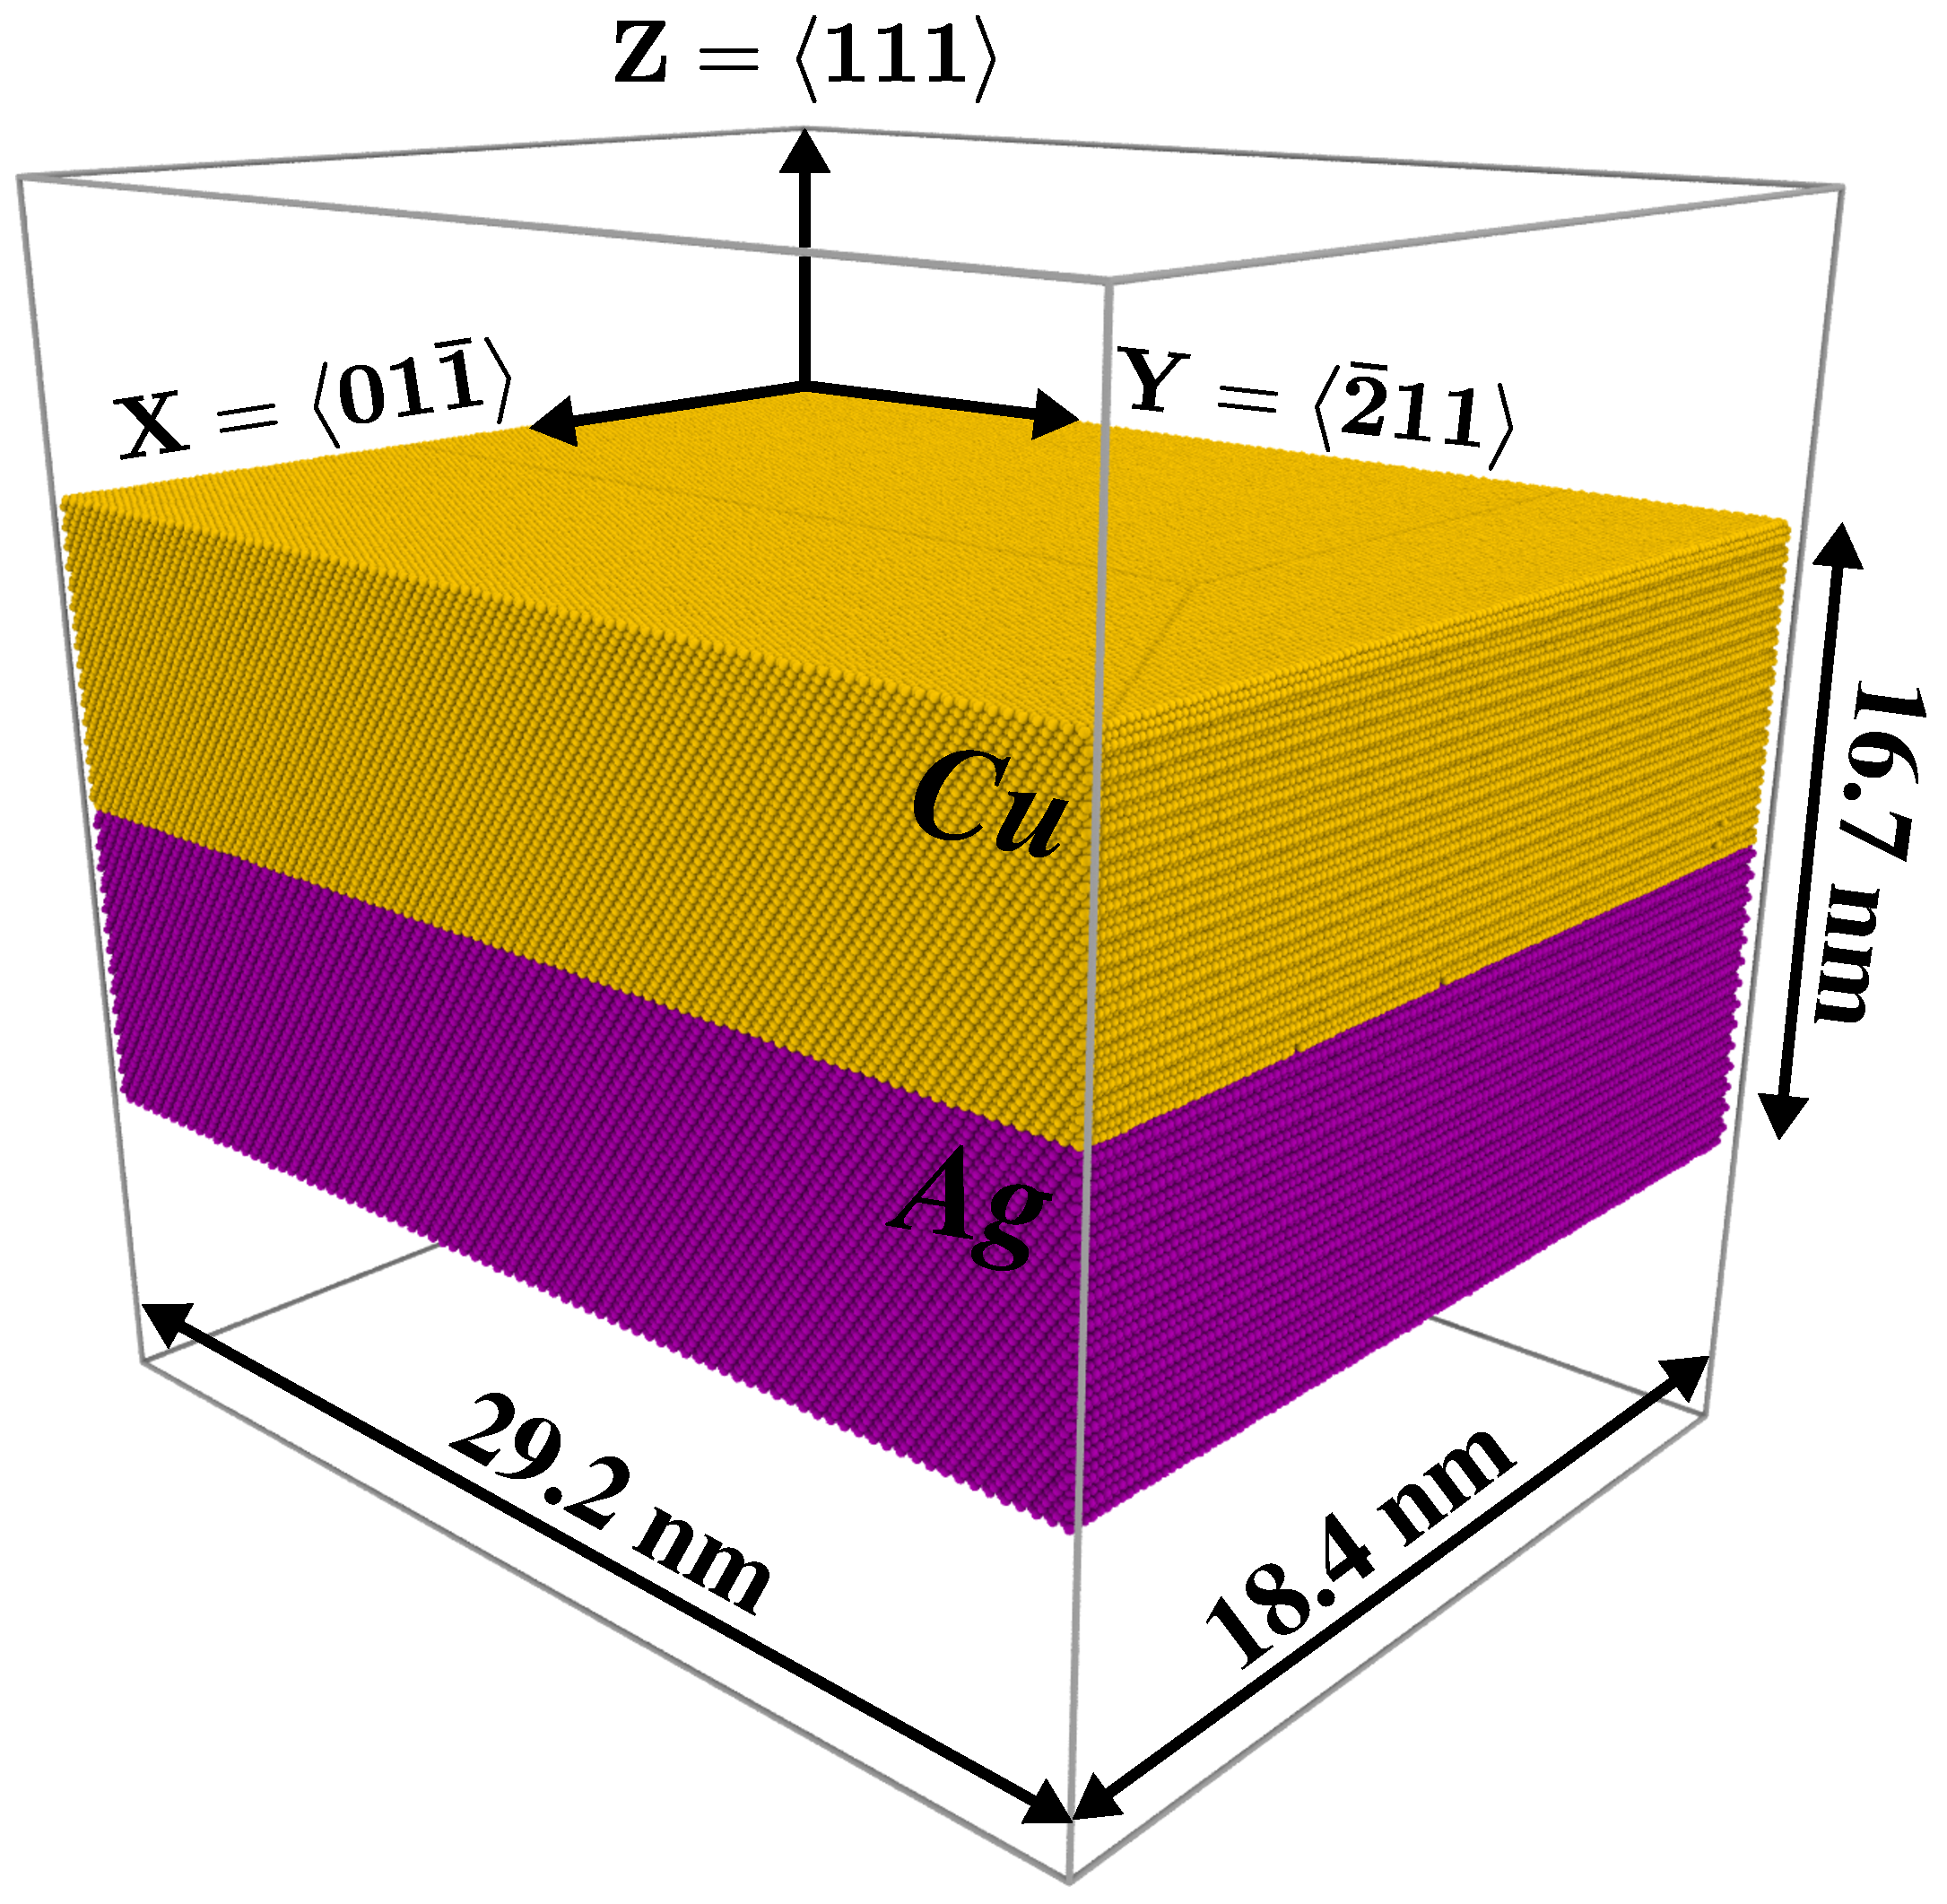
\includegraphics[width=70mm]{Pic/mod_geo.eps} 
	\end{center}
	\caption{Thin bimetallic film containing two layers of the same size. Atoms are coloured according to their types (Cu in purple and Ag in yellow).}\label{fig_mod_geo}
\end{figure}

Molecular dynamics calculations were then performed using the LAMMPS code \cite{plimpton95JCP}. The  embedded-atom method potential (EAM) of Williams et al. \cite{williams06MSMSE} was used to describe atomic interactions for Ag and Cu. For each of the two materials, this potential perfectly matches the lattice constants and closely reproduces the generalized stacking fault energies (GSFE) and the elastic constants, which are key parameters when one is interested in plasticity and more particularly in twin formation. Moreover for bimetallic materials, this potential also permits to describe interface sliding, which is quantified by the GSFE and the Peierls stress \cite{li15PM} at the $\lbrace111\rbrace$ Ag-Cu interface.

For each run, an energy minimization using a conjugate gradient algorithm was first performed to relax atomic positions at the interface. A 300 K temperature was then introduced by giving initial velocities to all atoms according to the Maxwell-Boltzmann distribution and the system was relaxed using an NPT integration according to the Nosé-Hoover thermostat, with zero pressure on each box faces. The system was subsequently compressed along the $Y=\langle\bar{2}11\rangle$ direction by deforming the simulation box at $\dot{\varepsilon}=10^{8}~$s$^{-1}$ constant strain rate and using an NVT integration at 300 K, with a time step of 1 fs.

Different sets of atoms initial velocities for a given configuration were used to obtain a reliable statistics from our simulations. Similar plasticity mechanisms were thus observed, showing a good reproducibility. A larger system with a different aspect ratio (33.4 nm x 41.8 nm x 20.0 nm, for $\approx$ 1993990 atoms) was also tested and similar results were obtained. 

Post-processing was performed, using the Open Visualization Tool (OVITO) to visualize the atomic configurations \cite{stukowski10MSMSE1}. The Dislocation Extraction Algorithm (DXA) was used to identify bulk and interface dislocations with their associated Burgers vector and an ``home-made'' algorithm based on local rotations was developed to identify twins. Note however that this algorithm, described in \ref{part_appendix}, can only identify primary twins.

	\subsection{Interface description}
	\label{subpart_interface}
 
Ag and Cu have a significantly different lattice parameter, respectively $a_{Ag}=4.1~\AA$ and $a_{Cu}=3.6~\AA$, which implies a high lattice mismatch of 12.1\%. The stress generated by this lattice mismatch is relaxed by misfit dislocations at the interface. For Ag-Cu multi layered materials only two semi coherent interfaces structures are possible: the cube on cube (COC) close-packed orientation and the twin orientation (TO). Both of them display a similar triangular mesh of misfit dislocations \cite{wang11SM,an15APL}.
\begin{figure}[!h]
	\begin{center}
		\includegraphics[width=70mm]{Pic/mod_inter.eps} 
	\end{center}
	\caption{Top view of Cu and Ag atoms along the interface(a.i) for a COC and (b.ii) for a TO interface. These views show the Shockley partial dislocations meshes (highlighted by the black lines), the associated triangular pattern (white segments), and the stacking faults distribution at the interface. (b.i) A side view along the $X=\langle01\bar{1}\rangle$ direction shows coherent areas alternating with intrinsic stacking fault (ISF) areas in the case of a COC interface and (b.ii) twin faults areas successively in the Cu layer and in the Ag layer in the case of a TO interface. Atoms are coloured according to the centrosymmetry parameter.}\label{fig_mod_inter}
\end{figure}

To introduce the COC interface in our model, we construct two slabs, one for each material. Ag and Cu layers are therefore aligned along the $Z=[111]$ direction while the crystal orientations of both slabs are $X=[01\bar{1}]$ and $Y=[\bar{2}11]$. The TO interface is built by keeping the previous orientation for the Ag layer while the Cu slab is rotated by 180° around the Y axis, leading to the following orientations: $X=[0\bar{1}1]$, $Y=[\bar{2}11]$ and $Z=[\bar{1}\bar{1}\bar{1}]$. It can be noted that the Cu lattice is almost matching the Ag lattice since $8.a_{Ag}\simeq9.a_{Cu}$. We can therefore adjust the global simulation box size by choosing initial lengths scaled to the average between $8.a_{Ag}$ and $9.a_{Cu}$, that is multiple of $\frac{\sqrt{2}}{2}\frac{(8.a_{Ag}+9.a_{Cu})}{2}$ in the $X=\langle01\bar{1}\rangle$ and $\frac{\sqrt{6}}{6}\frac{(8.a_{Ag}+9.a_{Cu})}{2}$ in the $Y=\langle\bar{2}11\rangle$ \cite{li15PM}. 

Doing so, misfit dislocations are then directly introduced at the interface but without any core structure relaxation. The interface is therefore relaxed by performing an energy minimization using the conjugate gradient method while keeping zero pressure on each box faces. Fig. \ref{fig_mod_inter}.a shows the triangular mesh of intersecting dislocations obtained, for both interface types. The three types of dislocations introduced are identified as Shockley partial dislocations, with Burgers vectors $\delta A$, $\delta B$ and $\delta C$ (according to the Thomson tetrahedron notation  \cite{hirth82book}) contained in the interface plane. These partial dislocations induce planar stacking faults at the interface. Depending on the interface type (COC or TO) the stacking faults are not similar and are differently distributed, as displayed in the side view of fig. \ref{fig_mod_inter}.b. The COC interface is composed of purely coherent areas alternating with intrinsic stacking fault (ISF) areas (Fig. \ref{fig_mod_inter}.b.i.), whereas the TO interface is entirely composed of twin faults with the faulted areas successively in the Cu layer and in the Ag layer (Fig. \ref{fig_mod_inter}.b.ii.).

\section{Influence of the interface type on mechanical twinning}
\label{part_influence}

Bimetallic systems with each type of interface were submitted to uni axial compression along the $Y$ axis, as described in section~\ref{subpart_model}. The tests detailed in section~\ref{subsubpart_sAg} and \ref{subsubpart_sAg2} were realised with two mono atomic steps on the Ag surface, separated by 14.7 nm. 
Typical deformation sequences are displayed in Fig.~\ref{fig_s1AgCOC}, with corresponding curves in Fig.~\ref{graph_stssnat}. Note however that because of thermal agitation, some variance in the systems behaviours can be observed.
In section~\ref{subsubpart_comparaison}, different nucleation sites were considered.

 
	\subsection{Cube on cube interface}\label{subsubpart_sAg}

\begin{figure*}[!t]
	\begin{center}
		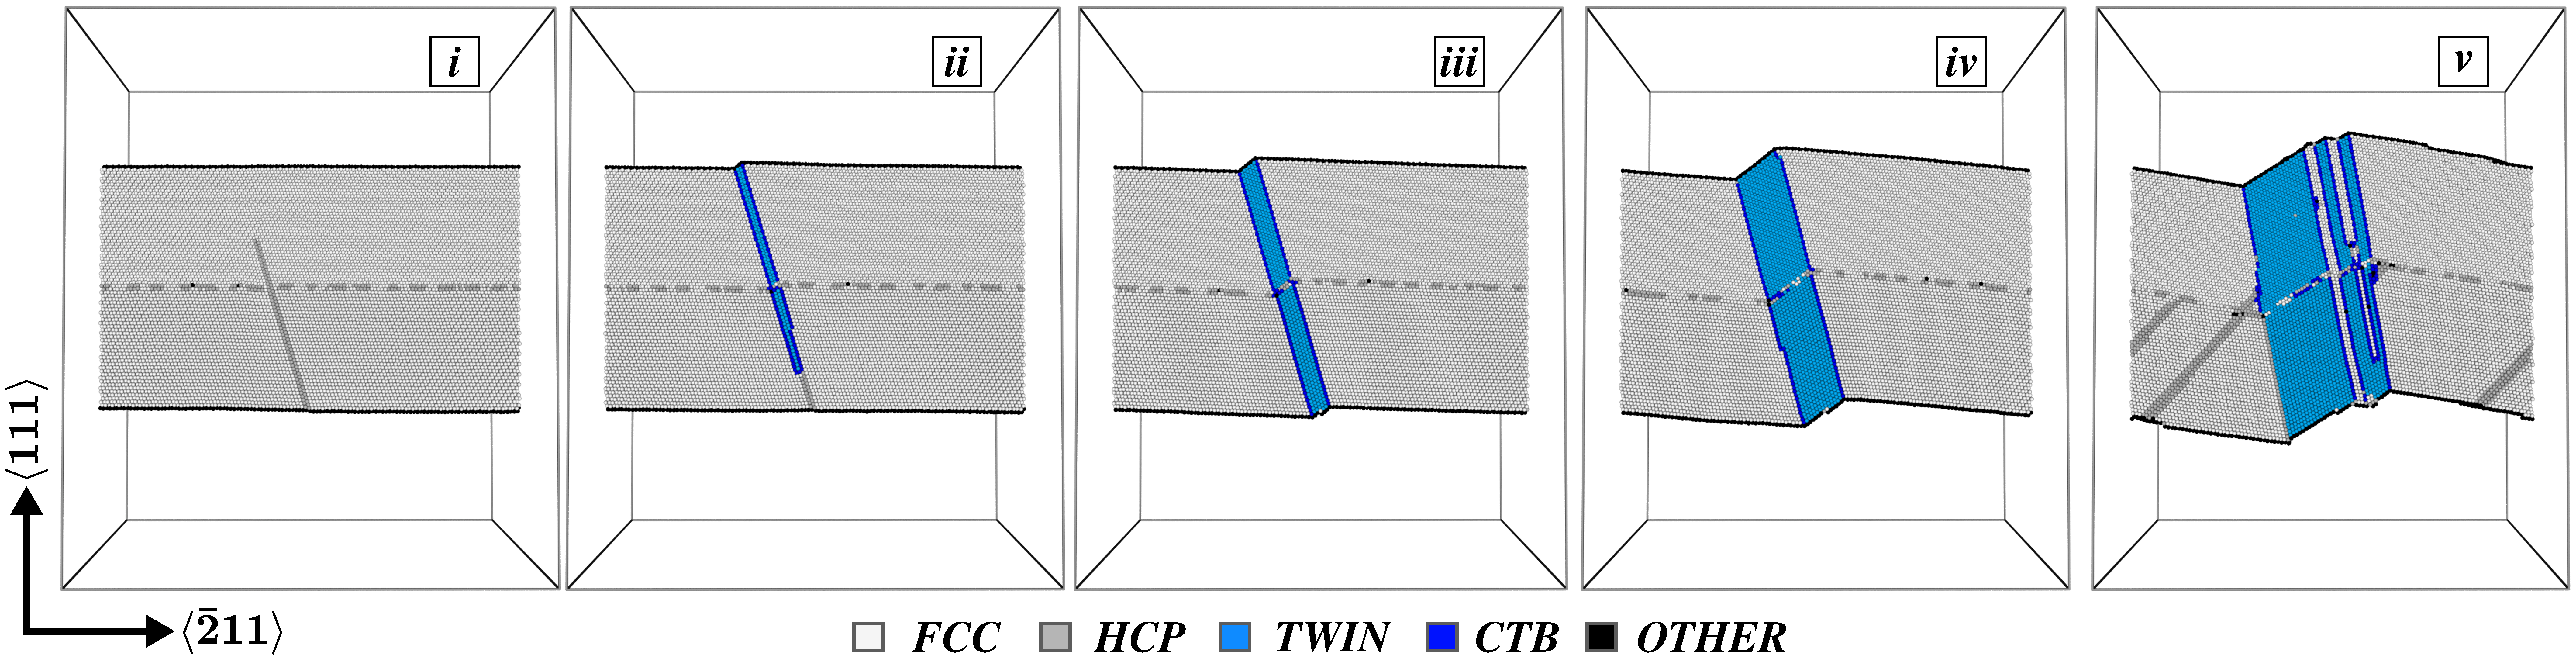
\includegraphics[width=165mm]{Pic/fig_s1AgCOC.eps} 
	\end{center}
	\caption{Plastic response of a thin Cu/Ag bimetallic film containing a COC interface under compression. (i-iii) Twin nucleation from a step on the Ag surface and (iv) twin thickening from the interface. (v) Subsequent plasticity mechanisms with twins and perfect dislocations nucleation. Atoms are shaded according to the common neighbour analysis (CNA) parameter: atoms in black belong to a surface or a dislocation line, atoms in ISF and TB are in grey, and atoms in perfect FCC crystal arrangement are in light grey. Besides, atoms are coloured according to our home-made twin identification algorithm (\ref{part_appendix}): in light blue for atoms belonging to a twin and in navy blue for atoms in a TB.}\label{fig_s1AgCOC}
\end{figure*}
For the system containing a COC interface, the onset of plasticity occurs for an average strain of 3.2\%. This average, as well as all those given throughout section~\ref{part_influence}, is calculated  over all simulations performed in the same configuration with different initial sets of velocities. As expected, the first plasticity event is the nucleation of a Shockley partial dislocation from one surface step. This dislocation then glides, leaving behind an intrinsic stacking fault (ISF), through the whole Ag layer and crosses the interface (see Fig.~\ref{fig_s1AgCOC}.a.i). When this first dislocation reaches the Cu surface, two new Shockley partial dislocations are nucleated on both sides of the ISF, thus forming a small twin (see Fig. \ref{fig_s1AgCOC}.a.ii). This ``rebound'' or ``reflexion'' mechanism for twinning was first pointed out by Christian who extended the mechanism described by Frank for perfect dislocations gliding on a same $\lbrace111\rbrace$ plane \cite{hirth82book} to Shockley partial dislocations in adjacent planes \cite{christian51PRS}. Then twin extends via the nucleation from both surfaces of several Shockley dislocations in adjacent $\lbrace111\rbrace$  planes along the TDs, always according to a ``rebound" mechanism. These onsets of plasticity and twinning correspond to the first stress drop in the light-blue stress-strain curve in Fig.~\ref{graph_stssnat}.a. When the stress becomes too low, twinning stops spontaneously for an average applied strain of 3.6\%; the corresponding snapshot is shown in Fig. \ref{fig_s1AgCOC}.a.iii. In figure \ref{graph_stssnat}.b, the light-blue curve reports the proportion of atoms belonging to a twin, obtained with our home-made algorithm, versus applied strain. A first increase can be seen between 3.3\% and 3.6\% strain, consistent with the mechanisms observed in Fig.~\ref{fig_s1AgCOC}.a.i-iii. 

\begin{figure*}[!t]
	\begin{center}
		\includegraphics[width=110mm]{Pic/fig_s1AgTO.eps} 
	\end{center}
	\caption{Plastic response of a thin Cu/Ag bimetallic film containing a TO interface under compression. (a.i-iii) Twin nucleation from a step on the Ag surface and Lomer dislocation nucleation from the interface. (a.iii-) Twin formation from the interface in the Cu layer. (b) Zoom at the interface of snapshot (a.i) showing the interaction between a Shockley partial dislocation nucleated at the Ag surface and a misfit dislocation. (c) Zoom of snapshot (a.ii) showing Lomer dislocation formation in the Ag layer and a Shockley partial dislocation in the Cu layer. As in Fig.\ref{fig_s1AgCOC}, atoms are coloured according to the CNA parameter and to our twin identification algorithm.}\label{fig_s1AgTO}
\end{figure*}

The stress in the whole system increases anew until twinning starts again at 5.1\% strain, with the nucleation of twin partial dislocations from surfaces. Another stress drop can therefore be observed in the stress-strain curve (Fig.~\ref{graph_stssnat}.a), and the proportion of ``twinned'' atoms increases a lot (Fig.~\ref{graph_stssnat}.b). This ends at an applied strain of 5.4\%, for which the stress starts rising up again, though more slightly than before the stress drops. In the same time, the proportion of ``twinned'' atoms increases slightly. This is explained by the activation of a different twinning mechanism, for which surfaces are not involved and Shockley partial dislocations are nucleated from the interface (Fig.~\ref{fig_s1AgCOC}.a.iv). This mechanism is described in detail in section~\ref{subsubpart_twin}. As evidenced in Fig.~\ref{graph_stssnat}, it is ``slower'' than the ``rebound'' mechanism and it is not sufficient to completely relax the stress induced by the applied strain.

For the specific test shown in Fig.~\ref{fig_s1AgCOC}, the ``interface'' twinning mechanism is observed after two sequences of ``surface'' twinning mechanism, with two stress drops in the stress-strain curves. This global twinning sequence will be later noted SSI (for Surface Surface Interface). It is worth noting that for other tests (about half of the runs) the ``interface'' twinning mechanism is observed after only one ``surface'' twinning mechanism sequence; this is evidenced by only one stress drop in the stress-strain curve, and no plateau in the ``twinned'' atoms proportion curve. This twinning sequence is then denoted SI.

Finally at higher applied strain (above 7.0\%), the stress is relaxed through the activation of other slip systems, with both Shockley partial and perfect dislocations (Fig.~\ref{fig_s1AgCOC}.a.v). These plasticity events are  accompanied by a stress drop and a significant increase of the proportion of ``twinned'' atoms (Fig.~\ref{graph_stssnat}).

	\subsection{Twin orientation interface}\label{subsubpart_sAg2}
	
The simulation was then performed for a thin film containing the TO interface. The onset of plasticity is similar to that observed with a COC interface: nucleation of a Shockley partial dislocation from one surface step for a same average strain of 3.2\% (see small stress drop in the red curve in Fig.\ref{graph_stssnat}.a). This is easily explained by the fact that the nucleation mechanism is very localized at the surface so that the interface plays no role in it. The dislocation then glides through the Ag crystal leaving behind an ISF, but unlike for the COC interface it is stopped and stored at the interface (Fig.~\ref{fig_s1AgTO}.a.i). However, in the absence of any other plasticity mechanism, the stress in the whole system increases again.
 
\begin{figure*}[!t]
	\begin{center}
		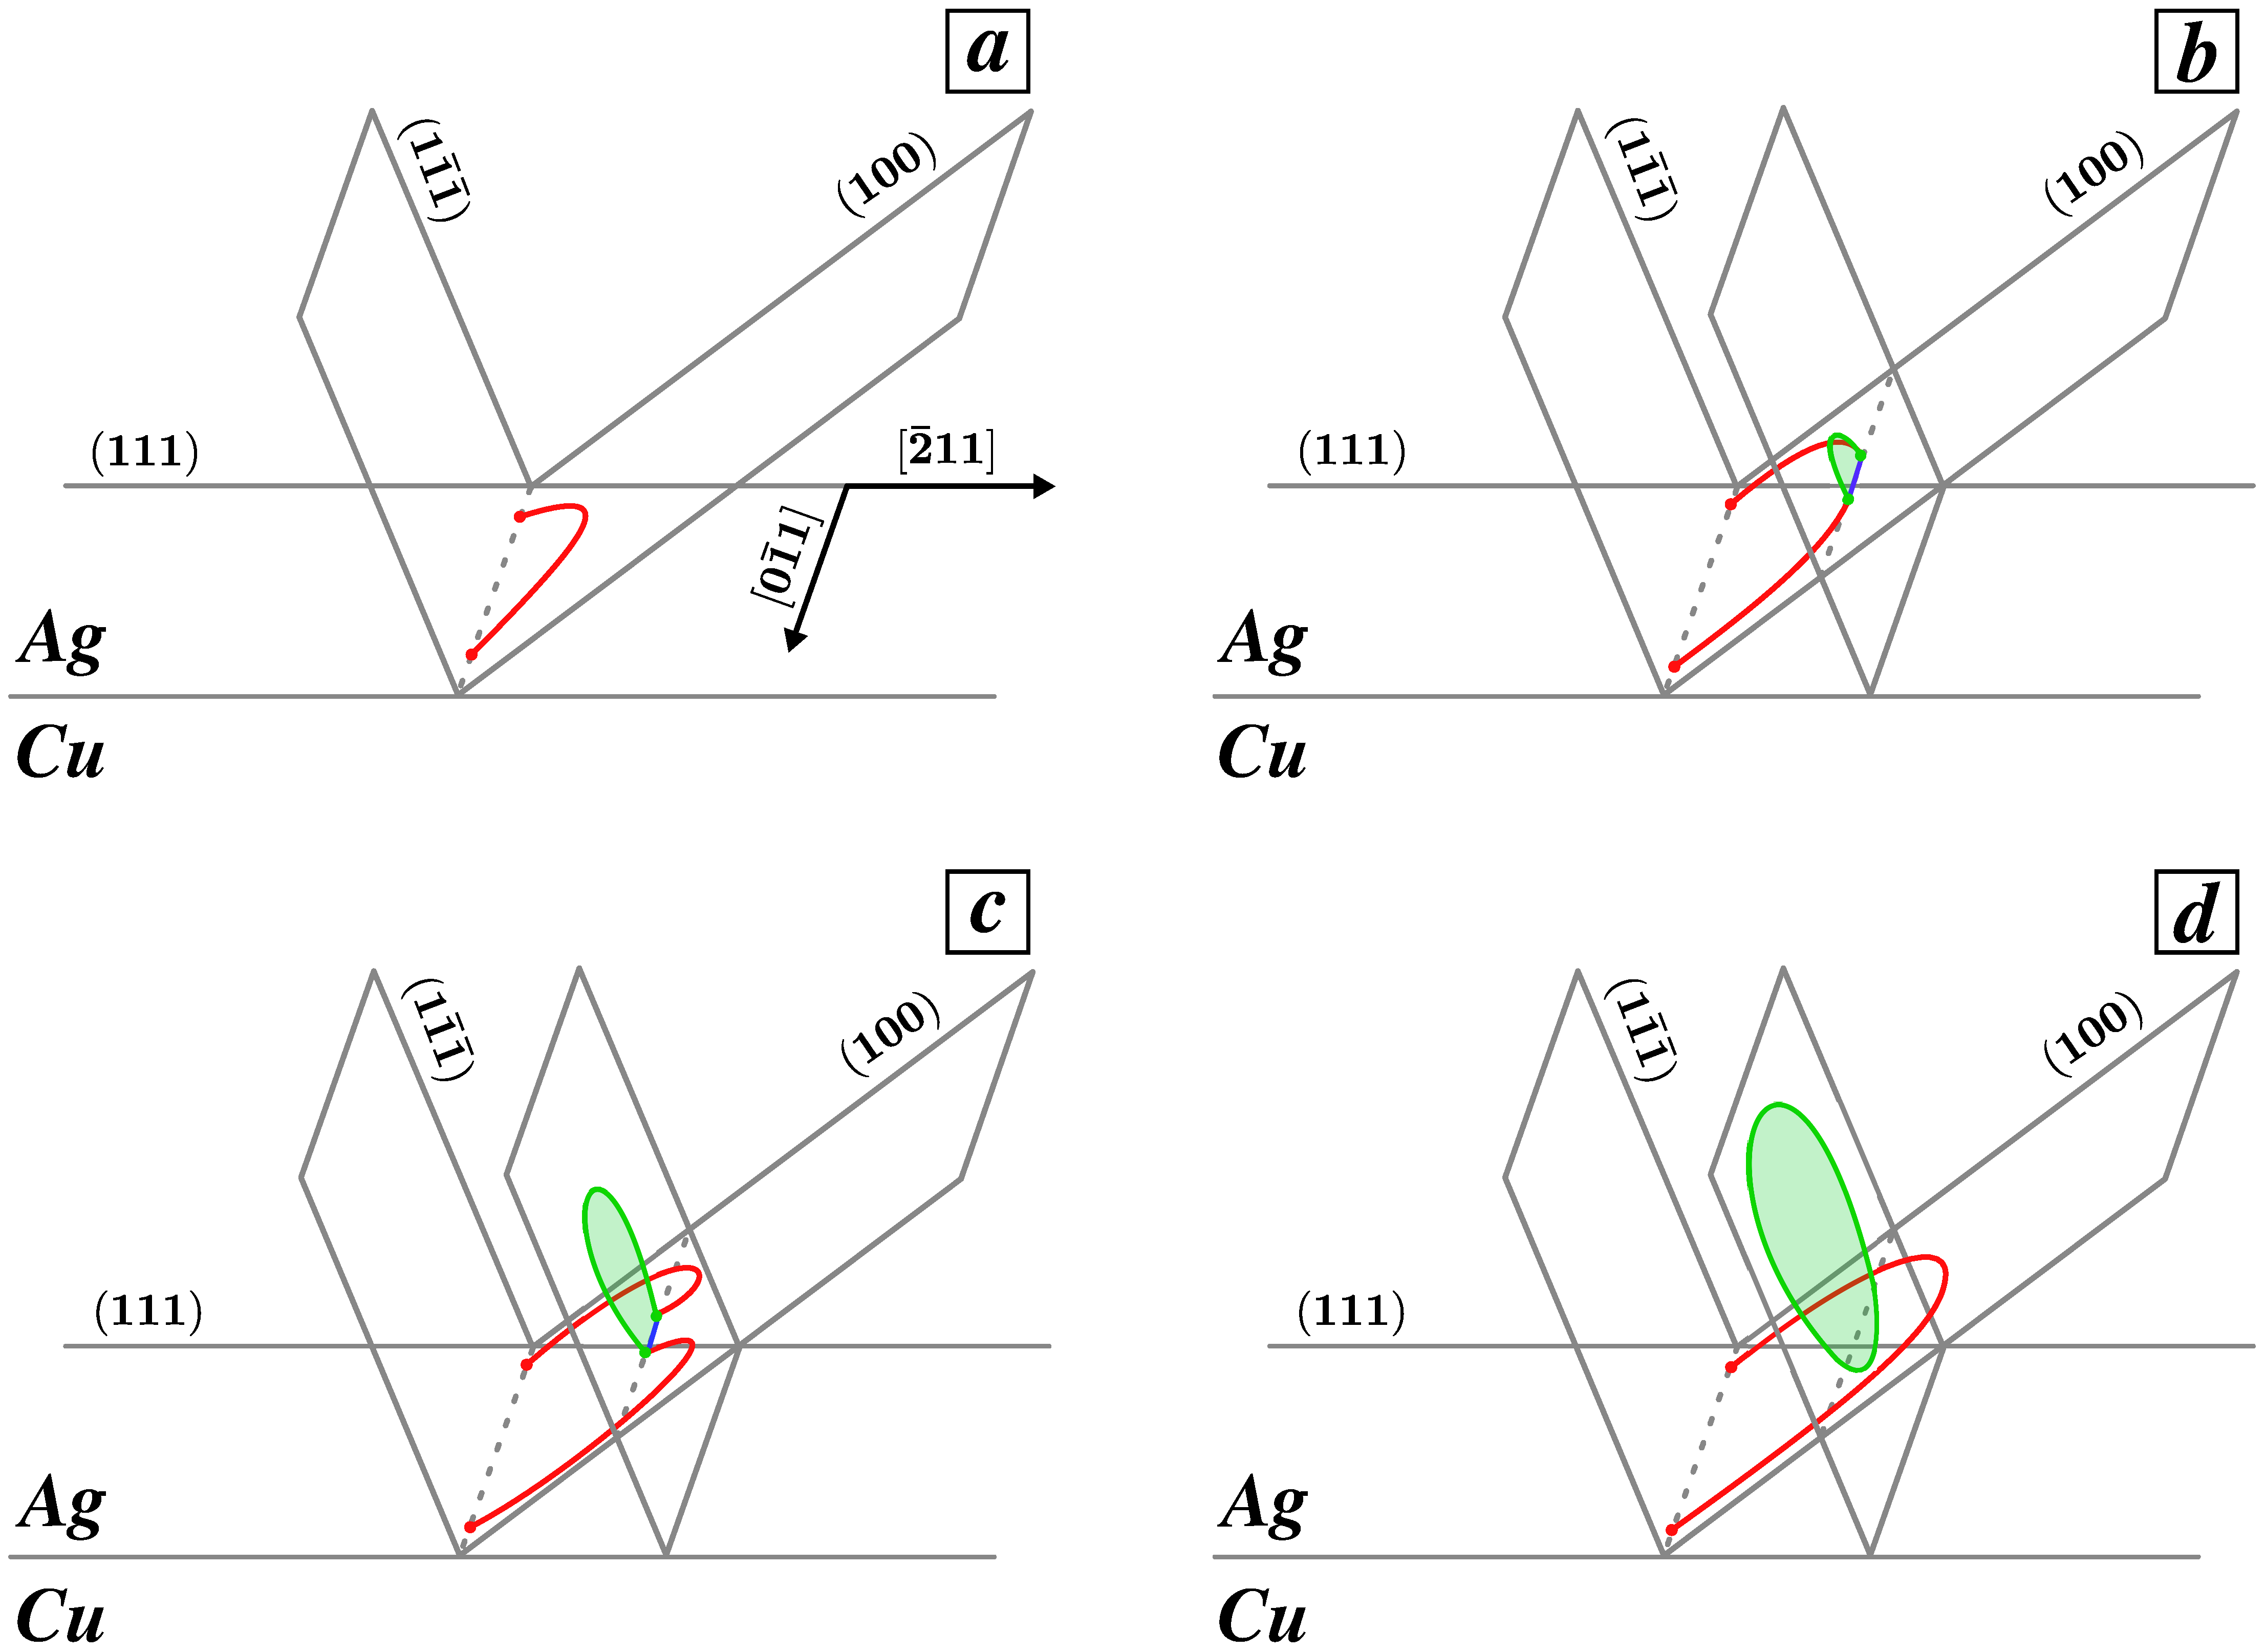
\includegraphics[width=110mm]{Pic/fig_lomdisso.eps} 
	\end{center}
	\caption{Schematic views of the mechanism leading to the formation of an isolated Shockley dislocation loop from a Lomer dislocation. (a) Starting configuration: Lomer dislocation (red line) gliding in a $(100)$ plane. (b) Lomer dissociation (equation~\ref{1}) into a Shockley partial dislocation in a $(1\bar{1}\bar{1})$ plane (green line) leaving behind an ISF (transparent green area) and a sessile Frank partial dislocation (blue line). (c) Extension of the Shockley and the Lomer dislocations, both being pinned by the sessile Frank dislocation. (d) Removal of the sessile Frank dislocation resulting in the formation of an isolated Shockley dislocation loop and release of the initial Lomer dislocation.}\label{fig_Lomer}
\end{figure*} 

Plasticity starts again for an average strain of 5.5\%, as shown in Fig.~\ref{fig_s1AgTO}.a.ii with the nucleation from the Ag surface of a Shockley partial dislocation forming a twin with the first nucleated dislocation. Right after (or for some tests right before), a Lomer dislocation in the Ag layer and a Shockley dislocation in the Cu layer are nucleated simultaneously from the interface (Fig. \ref{fig_s1AgTO}.a.ii). The mechanism through which the first Shockley partial dislocation interacts with the interface leading to the formation of a Lomer dislocation in Ag and a Shockley dislocation in Cu is explained in detail in section~\ref{subsubpart_lomer}. 
Note that the Schmid factor is very high (0.47) for the Lomer dislocation, which promotes its gliding in the (100) plane.
As the Lomer dislocation crosses the entire Ag crystal from the interface to the surface, it causes the nucleation of several Shockley partial dislocations through successive occurrences of the mechanism illustrated in Fig~\ref{fig_Lomer}. Indeed, when gliding the edge portion of the Lomer dislocation aligned along $\left[01\bar{1}\right]$ can dissociate into a Frank and a Shockley dislocation (Fig.~\ref{fig_Lomer}.b), according to \cite{wu09AM}:
\begin{eqnarray}\label{1}
	\begin{array}{ccccc}
\frac{1}{2}\left[0\bar{1}\bar{1}\right] &\rightarrow &  \frac{1}{3}\left[1\bar{1}\bar{1}\right]&+& \frac{1}{6}\left[\bar{2}\bar{1}\bar{1}\right] \\
BD &\rightarrow &  B\beta &+& \beta D\\
	\end{array}
\end{eqnarray} 
using Thompson tetrahedron notation. 
The Shockley partial can glide easily in the $\left(\bar{1}11\right)$ plane whereas the Frank partial dislocation is purely sessile. So the Shockley, Frank and Lomer dislocations are pinned at triple nodes that can only move along the $\left[01\bar{1}\right]$ direction (Fig.~\ref{fig_Lomer}.c). As the Shockley and Lomer dislocations bow out in their respective planes, the distance between the two triple nodes decreases and the Frank segment finally disappears according to the reaction reverse to reaction~\ref{1}. The Shockley partial forms a loop, which extends in the whole crystal, and the Lomer dislocation is released (Fig.~\ref{fig_Lomer}.d). While it continues to glide in its (100) plane, the Lomer dislocation can thus generate other Shockley partials in parallel $\left(\bar{1}11\right)$ planes via the same mechanism, and can eventually lead to the formation of twins if these planes are adjacent (Fig.~\ref{fig_s1AgTO}.a.iii-iv). We observe that this mechanism operates few times while the Lomer dislocation crosses the Ag layer. Simultaneously, few Shockley dislocations are nucleated from the surface and along the first ISF in the Ag crystal, thus forming a twin (Fig.~\ref{fig_s1AgTO}.a.ii-iv). In the Cu layer, the Shockley dislocation reaches the surface and induces the nucleation of new Shockley dislocations in $\lbrace111\rbrace$ adjacent planes, thereby forming a twin (Fig.~\ref{fig_s1AgTO}.b.iii-iv). All the formed twins are finally stopped at the interface.

\begin{figure*}[!t]
	\begin{center}
		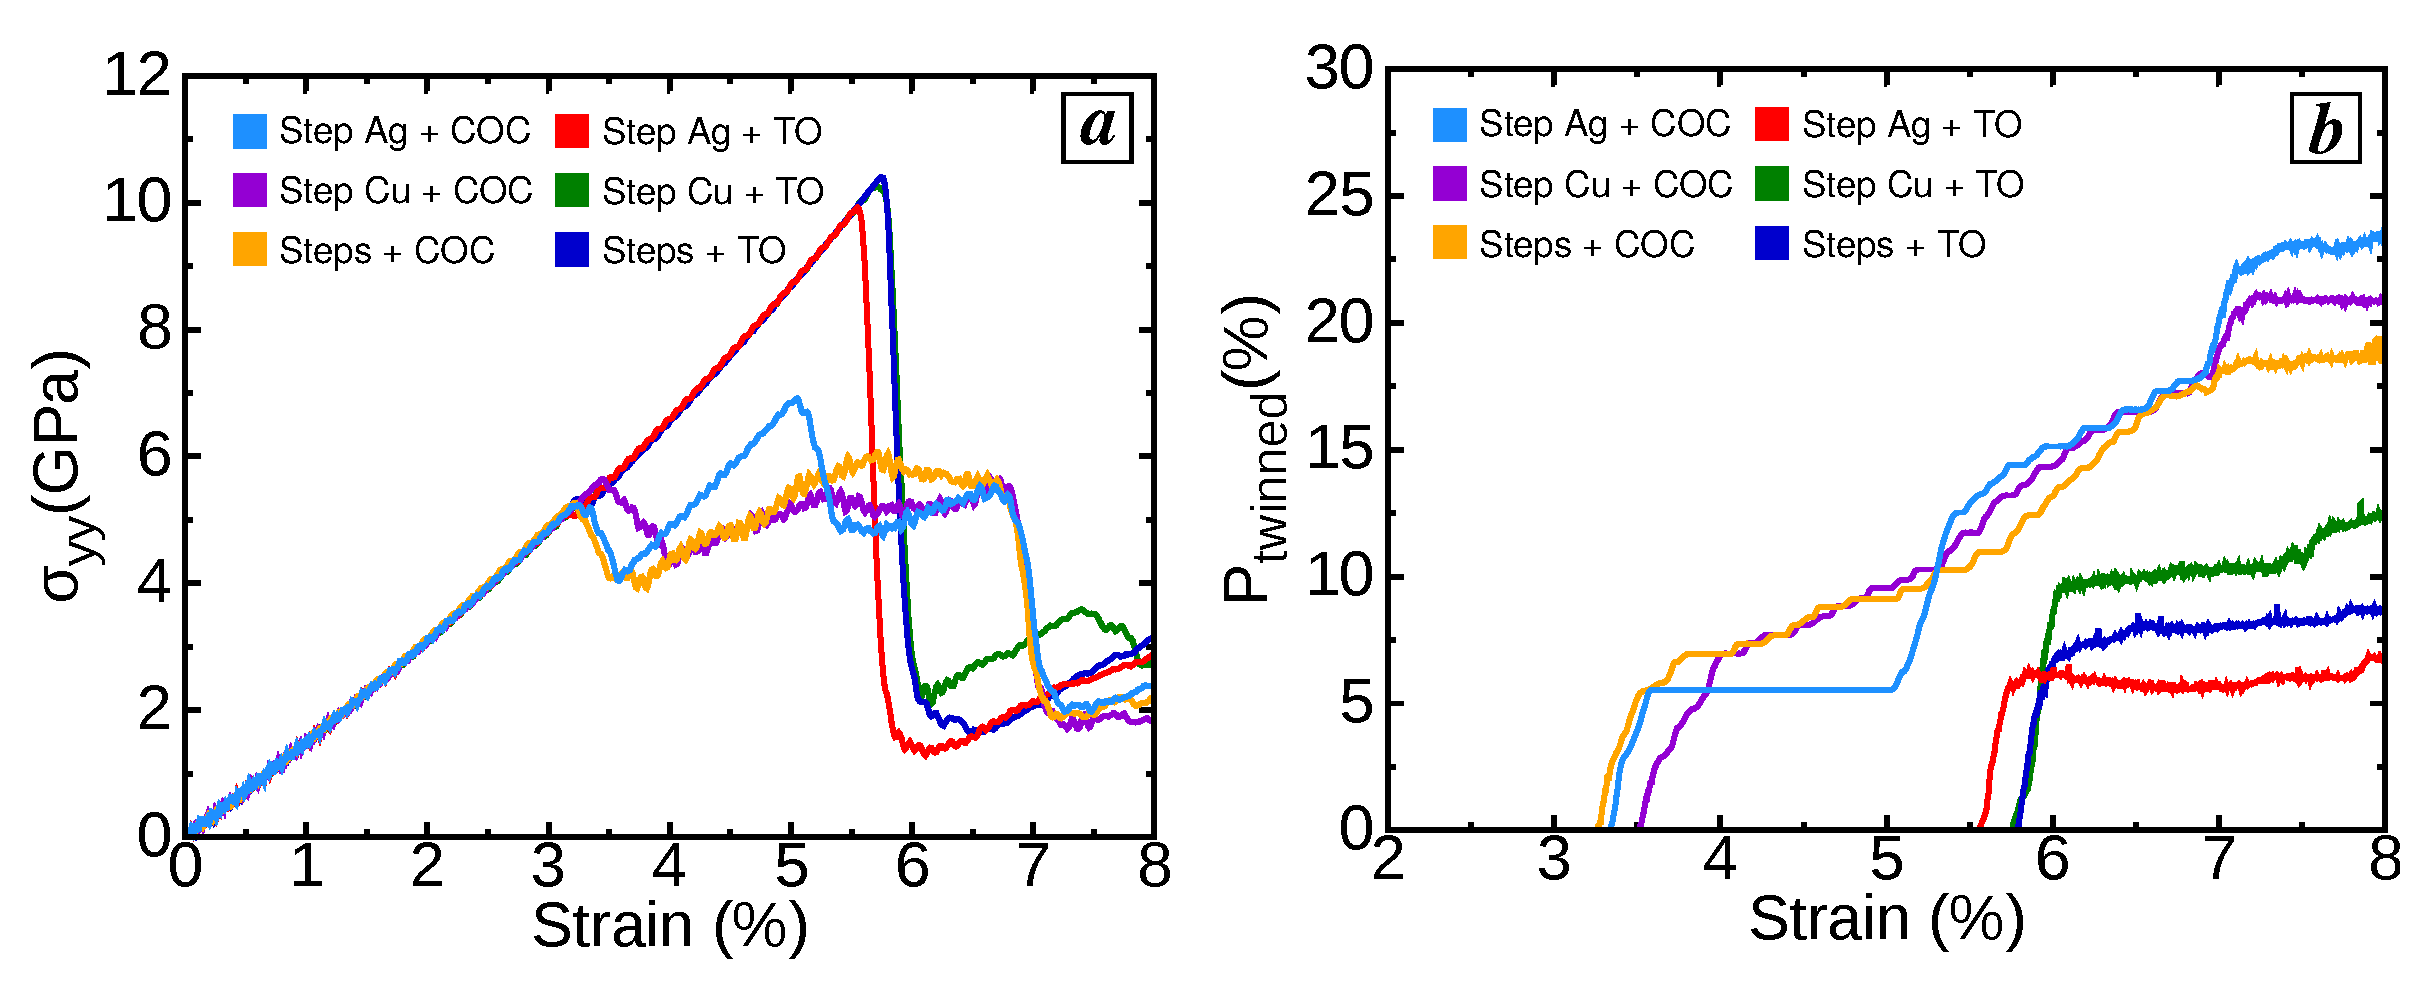
\includegraphics[width=150mm]{Pic/graph_natstss.eps} 
	\end{center}
	\caption{(a) Stress - strain curves and (b) total proportion of atoms belonging to a twin as a function of strain. Light blue, purple and yellow curves correspond to film configurations containing a COC interface and with respectively surface steps on the Ag, Cu and both surfaces. Finnaly, red, green and navy blue curves correspond to film configurations containing a TO interface and with respectively surface steps on the Ag, Cu and both surfaces.}\label{graph_stssnat}
\end{figure*}

These plasticity mechanisms all operate at the same time at 5.5\% applied strain, resulting in an important stress drop which can be seen in the stress-strain curves (red curve in Fig. \ref{graph_stssnat}.a). There is also a significant increase of the ``twinned'' atom proportion because of the concomitant nucleation of twins in the Cu and Ag layers (red curve in Fig. \ref{graph_stssnat}.b), although the proportion of ``twinned'' atom is much less than for a COC interface at the same applied strain.
 
	\subsection{Varying nucleation sites}\label{subsubpart_comparaison}
	
In order to test the influence of the first plasticity event location, steps were introduced on the Cu surface, along with or without steps on the Ag surface.
	
For all tested cases, Shockley dislocations are nucleated from   steps. When steps are introduced on the Cu surface only, the yield point is slightly higher ($\sim 3.3\%$) than when steps are present on the Ag surface. This is consistent with higher intrinsic and unstable stacking fault energies in Cu. When steps are introduced on both surfaces, the first plasticity event therefore always starts at one of the Ag surface step, and the yield point is similar to that described in sections~\ref{subsubpart_sAg} and \ref{subsubpart_sAg2} (yellow and navy-blue curves in Fig.~\ref{graph_stssnat}.a). 

For systems with a COC interface, the plastic response to the applied strain is similar whatever the first dislocation nucleation site. The two distinct twinning mechanisms (surface ``rebound'' and interface nucleation) are observed, but the twinning sequence can be different: SSI or SI (see section~\ref{subsubpart_sAg}). It is worth noting that if steps are present on the Cu surface only, the ``interface'' twinning mechanism is always activated after only one ``rebound'' mechanism sequence (see purple curves in Fig.~\ref{graph_stssnat}), according to a SI twinning sequence. As it will be discussed in section~\ref{subsubpart_twin}, this is partly due to a higher yield strain. It should also be noted that when steps are introduced on both sides, the onset of plasticity in Ag is quickly followed by twin formation which relaxes a significant amount of stress (see yellow curve in Fig.~\ref{graph_stssnat}.a), so that the steps on the Cu surface are in general not activated.

For systems containing a TO interface, the onset of plasticity is not strongly influenced by the location of the first nucleated dislocation: Shockley partial dislocations are always first nucleated from surface steps, glide through half part of the system and are stopped and stored at the interface. If surface steps are present on both sides of the system, this occurs almost simultaneously in both Cu and Ag parts; two Shockley dislocations are thus nucleated.
As for the subsequent events, they depend significantly on the first nucleation sites: Lomer dislocations are formed only in the Ag crystal, when a Shockley partial in the Ag layer interacts with the interface. When steps are introduced on the Cu surface only, the first Shockley dislocation nucleates from the step in the Cu crystal. A new Shockley partial can later be nucleated from a random site on the Ag surface, for high enough accumulated stress. Then it glides and reaches the interface where its interaction with misfit dislocations gives rise to Lomer dislocation and another Shockley partial according to the mechanism described in section~\ref{subsubpart_sAg2}.
 
\section{Role of misfit dislocations}
\label{part_misfit}

In section~\ref{part_influence}, it has been evidenced that interfaces are not involved in the onset of plasticity (first dislocation nucleation), which occurs at surfaces. However, interactions between Shockley dislocations or TB and interface misfit dislocations can lead to specific plasticity mechanisms. In particular, in section~\ref{subsubpart_lomer} we describe the Lomer dislocation nucleation mechanism observed for the TO interface (see section~\ref{subsubpart_sAg2}). Similarly, the twinning mechanism operating from the interface and contributing to the twin extension in the case of a COC interface (see section~\ref{subsubpart_sAg}) is detailed in section~\ref{subsubpart_twin}.  

	\subsection{Nucleation of Lomer dislocation - TO interface}
	\label{subsubpart_lomer}
	
In the case of a TO interface, dislocation transmission is not possible due to an high angle disorientation between the two layered crystals. Dislocations nucleated from the surface of the film are therefore stopped and stored at the interface. These Shockley partial dislocations can therefore combine with misfit dislocations (Fig. \ref{fig_s1AgTO}.b), according to the following reaction:

\begin{eqnarray}\label{2}
	\begin{array}{ccccccccccccc}
\frac{1}{6}\left[211\right]_{Ag} &+& \frac{1}{6}\left[2\bar{1}\bar{1}\right]_{Ag} &\rightarrow& \frac{2}{3}\left[100\right]_{Ag},\\
D\beta_{Ag} &+& B\delta_{Ag} &\rightarrow& \frac{2}{3}BD/AC_{Ag} 
	\end{array}
\end{eqnarray}

When the accumulated stress is high enough, the newly formed dislocation dissociates according to the reaction:

\begin{eqnarray}\label{3}
	\begin{footnotesize}
	\begin{array}{cccccccc}
\frac{2}{3}\left[100\right]_{Ag} &\rightarrow& \frac{1}{2}\left[0\bar{1}\bar{1}\right]_{Ag} &+& \frac{1}{6}\left[\bar{2}\bar{1}\bar{1}\right]_{Cu}  &+& \\
 & & \frac{1}{6}\left[2\bar{1}\bar{1}\right]_{Ag} &+& D_{res}, \\
\frac{2}{3}BD/AC_{Ag} &\rightarrow& BD_{Ag} &+& \beta D_{Cu} \\
 & & B\delta_{Ag} &+& D_{res}
	\end{array}
 	\end{footnotesize}
\end{eqnarray}
where $BD_{Ag}$ is a Lomer dislocation gliding in the Ag layer, $\beta D_{Cu}$ is a Shockley partial dislocation gliding in the Cu layer, $B\delta_{Ag}$ is the initial recovered interfacial misfit dislocation and $D_{res}$ is a residual interfacial dislocation (Fig. \ref{fig_s1AgTO}.c). The Shockley partial dislocation then crosses the entire Cu layer and induces the formation of a twin via the nucleation of successive Shockley dislocations from the free Cu surface. The interface thus directly plays the role of a source for twin nucleation. 

Another mechanism of dislocation recombination which can lead to the formation of a Lomer dislocation has been observed for some runs, when two Shockley partial dislocations are nucleated successively in $\lbrace111\rbrace$ adjacent planes in the Cu layer, thus forming an extrinsic stacking fault.These two Shockley dislocations collapse and form a super dislocation ($ 2~D\beta_{Cu} $).
The super dislocation rapidly dissociates into a sessile stair-rod dislocation ($\beta\delta_{Cu}$) stored at the interface and a Lomer dislocation $ BD_{Ag} $ which glides in a $\lbrace100\rbrace$ plane in the Ag layer, according to the reaction:

\begin{eqnarray}\label{4}
	\begin{array}{ccccc}
\frac{1}{3}\left[211\right]_{Cu} &\rightarrow & \frac{1}{6}\left[011\right]_{Cu} &+& \frac{1}{2}\left[0\bar{1}\bar{1}\right]_{Ag}, \\
2~D\beta_{Cu} &\rightarrow & \beta\delta_{Cu} &+& BD_{Ag} \\
	\end{array}
\end{eqnarray}

In any case, for the TO interface, dislocation-interface interactions always lead to the nucleation of Lomer dislocations. Lomer dislocations have already been observed experimentally \cite{bonneville90PML,mills89PMA}, and in few simulations of deformed FCC metals it has been found that they usually result from the interaction of a perfect dislocation and a TB \cite{wu09AM,sansoz07NL}. However, they are not stable and when it is possible they generally dissociate and form Lomer-Cottrell lock \cite{hirth82book,wu09AM}. In our systems, the dissociation mechanism is not or only partially occurring, as seen in section~\ref{subsubpart_sAg2}. This is partly due to a high accumulated stress associated with an high Schmid factor which is sufficient to induce their easy gliding in $\lbrace100\rbrace$ planes. Furthermore due to the proximity of surfaces, dislocations are rapidly eliminated which reduces their dissociation probability while gliding. As described in section~\ref{subsubpart_sAg2}, Lomer dislocations can often act as sources for Shockley dislocations and possibly deformation twins. 

	\subsection{Twin dislocation nucleation induced by misfit dislocation - COC interface}\label{subsubpart_twin}
	
Unlike the TO interface, the COC interface is fully permeable to dislocations; interface-dislocations interactions are therefore very limited. However, as seen in section~\ref{subsubpart_sAg}, the interface can act as a source for TDs. This is always preceded by the formation of a twin via the dislocation ``rebound'' mechanism at the free surfaces. Therefore, due to this twin formation and the periodic boundary conditions, a rotation of the film around the $X=\langle01\bar{1}\rangle$ axis happens (Fig. \ref{fig_rotation}).
\begin{figure}[!h]
	\begin{center}
		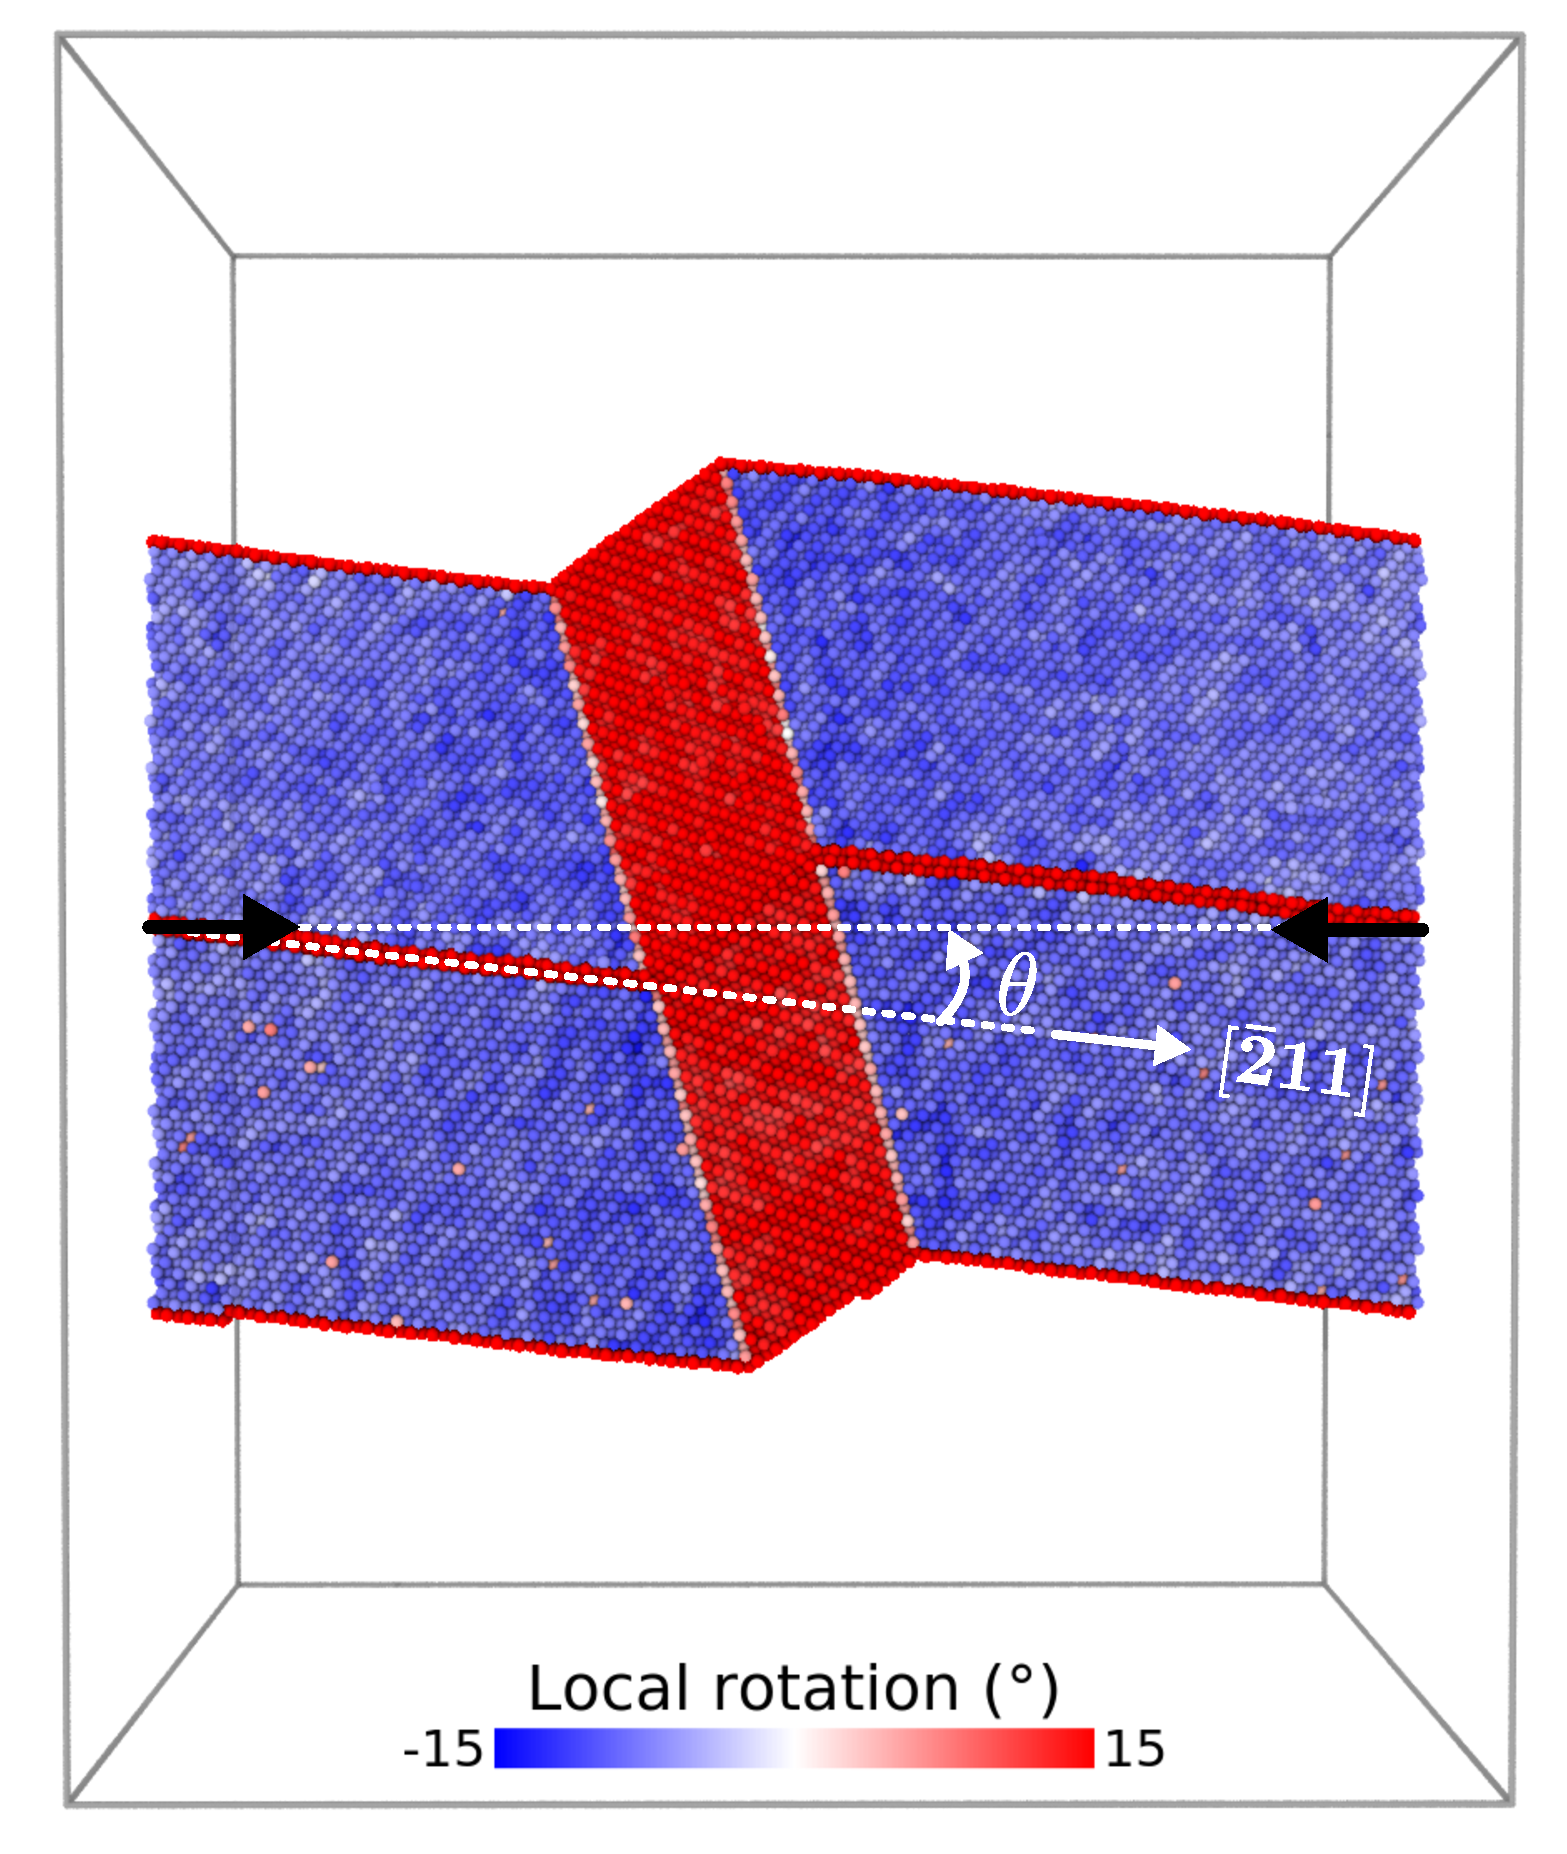
\includegraphics[width=70mm]{Pic/fig_rotation.eps} 
	\end{center}
	\caption{Thin Cu/Ag film containing a COC interface deformed plastically by twinning and rotated around the $X=\langle01\bar{1}\rangle$ axis with an angle $\theta$. Atoms are coloured according to the rotation of their local environment $\theta_{i}$ (compared to a non deformed initial configuration, see \ref{part_appendix}). Black arrows correspond to the compression axis deformation and the white arrow to the $[\bar{2}11]$ direction belonging to the interface plane.}\label{fig_rotation}
\end{figure}
\begin{figure*}[!t]
	\begin{center}
		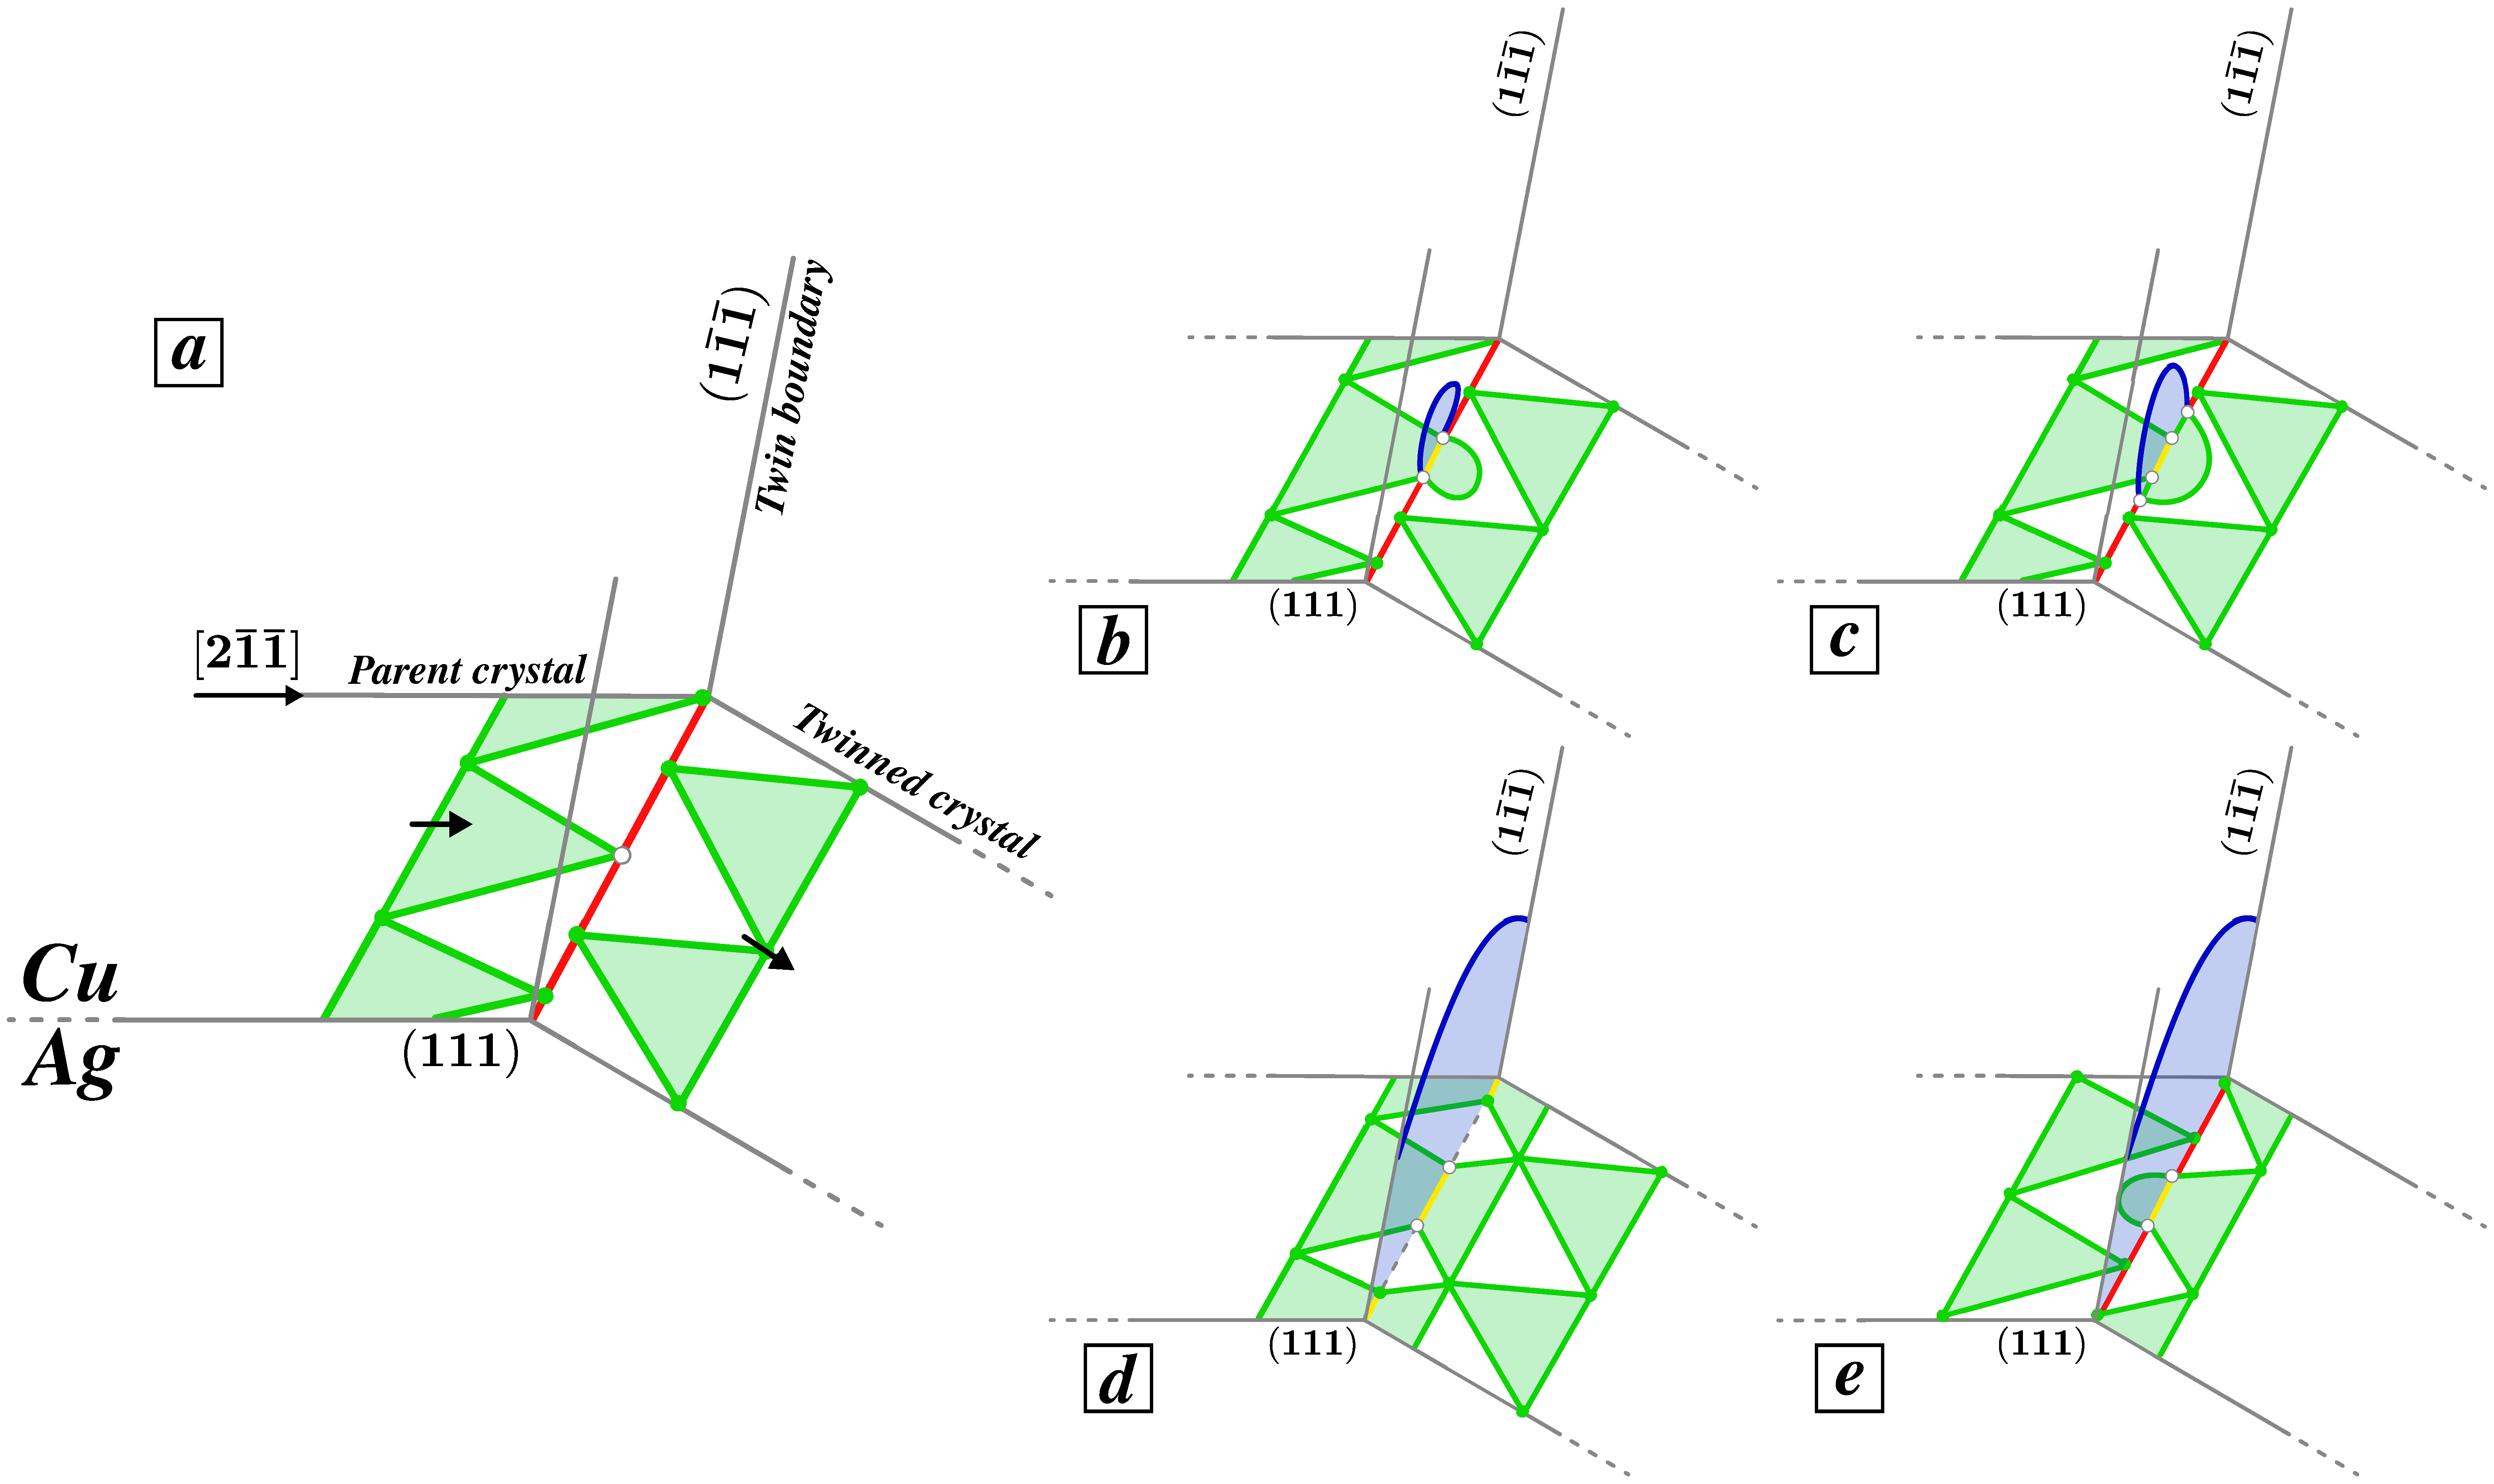
\includegraphics[width=160mm]{Pic/fig_ENT.eps} 
	\end{center}\caption{Schematic view of the interactions of misfit dislocations with a TB, leading to the nucleation of twin dislocation in the Ag layer. A full description of these interactions mechanisms is made in part \ref{subsubpart_twin}. The light green lines correspond to Shockley partial dislocations gliding along the interface plane with their associated ISF (green areas), whereas the blue line corresponds to one gliding along the TB plane and the blue area corresponds the ISF. The red line is associated to perfect lattice dislocation and the purple line to a residual dislocation blocked along the interface and the TB plane. The black arrows in (a) indicate the direction of the misfit dislocations motion.}\label{fig_ENT}
\end{figure*}
\begin{figure*}[!t]
	\begin{center}
		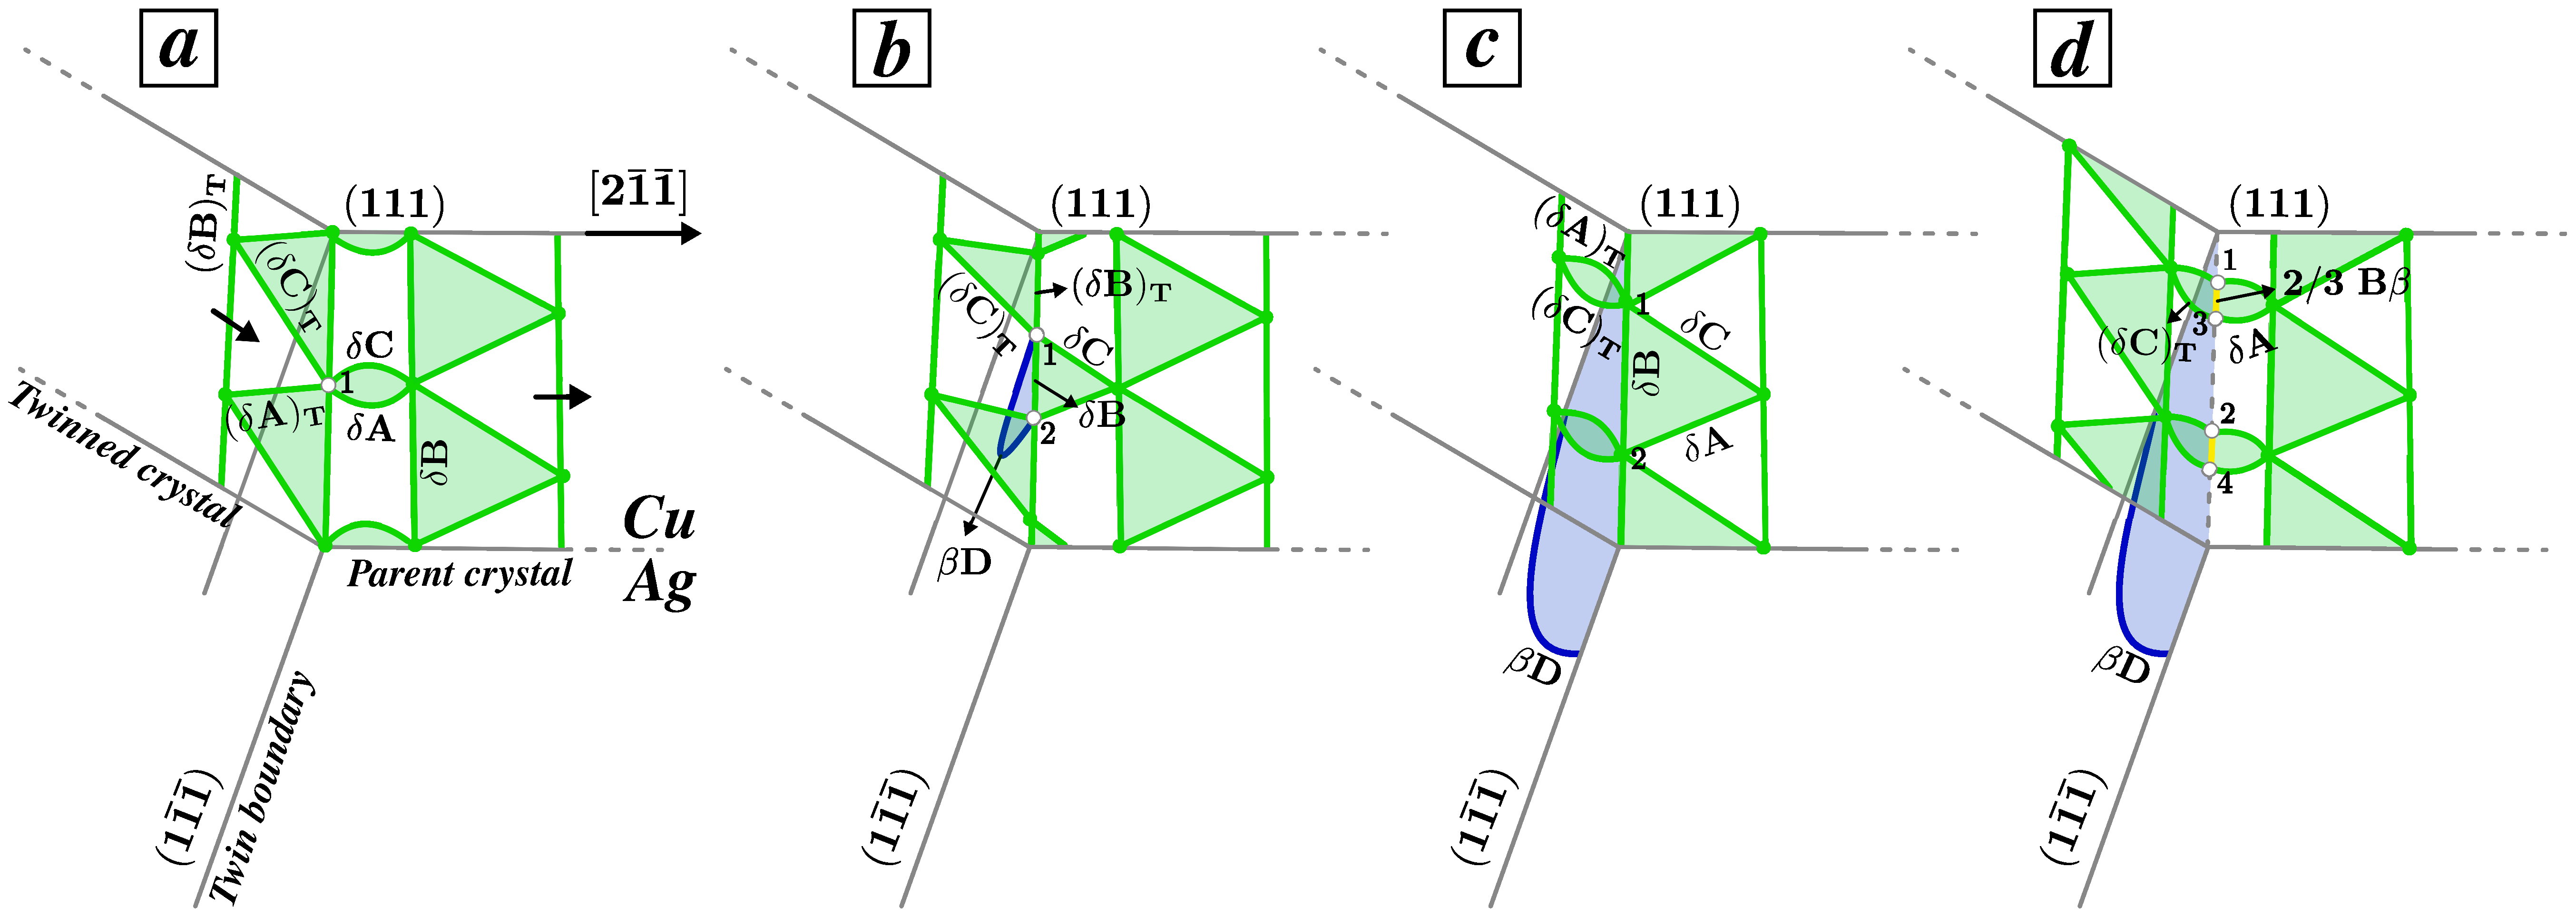
\includegraphics[width=160mm]{Pic/fig_SOR.eps} 
	\end{center}\caption{Schematic views of the exit of the misfit dislocations pattern from the twin, leading to the nucleation of a TD in the Cu layer (see text for details). The lines colour coding is the same as that of Fig.~\ref{fig_ENT}. The black arrows in (a) indicate the direction of the misfit dislocations motion.}\label{fig_SOR}
\end{figure*}
The resolved shear stress in the interface plane (which was initially close to 0~GPa) then increases sufficiently to induce gliding of misfit dislocations. They therefore glide inside the interface until being stopped at the newly formed TB, where they interact with the latter. This interaction gives rise to the nucleation of a TD, as detailed below. Similarly, the resolved shear stress along the interface inside the twin is not zero, so that misfit dislocations also glide inside the twinned part. They then interact with the second TB when they participate to the twin extension. Therefore, two mechanisms (one at each TB) lead to the extension of the newly nucleated twin. The first one, displayed in Fig.~\ref{fig_ENT}, corresponds to the entry of the whole misfit dislocations pattern inside the twin, thus crossing one of the TB. For the description, we choose to start with the initial configuration shown in Fig~\ref{fig_ENT}.a. This is actually not the real starting configuration, because when the twin is formed the position of the TB does not perfectly match with a specific component of the misfit dislocations pattern. The real configuration after the first (``rebound'') twinning mechanism corresponds to that of Fig.~\ref{fig_ENT}.d, but we can assert that at some time during the process the  configuration of Fig.~\ref{fig_ENT}.a will be reached without the emission of any TD.

Starting from the configuration displayed in Fig~\ref{fig_ENT}.a, the gliding of the misfit dislocations mesh across the TB is first accompanied by a reaction at node 1, producing a twinning  Shockley dislocation gliding in the Ag layer along the TB ($D\beta$, blue line), an interfacial misfit dislocation inside the twin ($(\delta B)_T$, green line) and a residual interfacial dislocation stopped at the TB ($2/3 B\beta$, purple line), as shown in Fig.~\ref{fig_ENT}.b. The two  nodes 1 and 2 (Fig.~\ref{fig_ENT}.b), arising from the dissociation of node 1, move along the $\left[ 01 \bar{1} \right]$ line direction of the two perfect lattice dislocations ($BA$ and $BC$, red lines) locked at the intersection of the TB and the interface. While the TD $D\beta$ and the misfit dislocation $(\delta B)_T$ extend, node 1 (respectively 2) dissociates so as to form a new Shockley dislocation $(\delta A)_T$ (respectively $(\delta C)_T$) along the $\left[ 01\bar{1} \right]$ direction between nodes 1 and 3 (respectively between nodes 2 and 4), as shown in Fig.~\ref{fig_ENT}.c. The three Shockley dislocations $(\delta B)_T$, $(\delta A)_T$ and $(\delta C)_T$ between nodes 1-2, 1-3 and 2-4 respectively make up the sketch of the ``triangular'' ISF pattern inside the twin. As node 1 (respectively 2) moves along the $\left[ 01\bar{1} \right]$ direction, the perfect dislocation BA (respectively BC) progressively disappears until node 1 reaches node 5 (respectively node 2 reaches node 6). At this point, because of the periodicity of the interfacial pattern along the $\left[ 01\bar{1} \right]$ direction, node 5 is equivalent to node 2 (respectively node 6 is equivalent to node 1), so that nodes 1 and 2 recombine. The interfacial dislocation $(\delta B)_T$ between nodes 1 and 2 can thus glide freely along the interface inside the twin, and the twinning Shockley dislocation $D\beta$ can glide freely along the TB. 
The whole faulted ``triangular'' pattern then crosses the TB with misfit dislocations $(\delta A)_T$ and $(\delta C)_T$ transmitted through nodes 3 and 4, as indicated in Fig.~\ref{fig_ENT}.d. This leaves behind the residual dislocation $2/3 B\beta$ locked at the TB. Once the misfit Shockley partial dislocations $\delta C$ and $\delta A$ have gone through the TB, the last partial dislocation $\delta B$ (closing the ISF in the perfect crystal) reacts at nodes 3 and 4 with this residual dislocation, so as to form the perfect lattice dislocations $BC$ and $BA$ at the TB and allow the extension of misfit dislocations $(\delta A)_T$ and $(\delta C)_T$ inside the twin (Fig.~\ref{fig_ENT}.e). Nodes 3 and 4 finally recombine, thereby closing the triangular ISF pattern in the twinned crystal part. At the end of this process, the misfit dislocations pattern has entirely crossed the TB, the two perfect lattice dislocations $BC$ and $BA$ have been formed and regrouped in one initial node, and the whole system is therefore back into the initial configuration of Fig.~\ref{fig_ENT}.a. However, during this process a TD has been emitted in the Ag layer, thus contributing to the twin extension.

The second mechanism, displayed in Fig.~\ref{fig_SOR}, corresponds to the exit from the twin of the whole misfit dislocations pattern. Fig.~\ref{fig_SOR}.a shows the starting configuration for the description. As for the previous described mechanism, this configuration, though not being the real starting one, will necessarily be reached during the process. From this configuration, the first step is a reaction at node 1 (Fig.~\ref{fig_SOR}.a), producing the TD $\beta D$ (blue line in Fig.~\ref{fig_SOR}.b) in the Cu layer and the misfit dislocation $\delta B$ along the $\left[ 01\bar{1} \right]$ direction between nodes 1 and 2 (Fig.~\ref{fig_SOR}.b), arising from the dissociation of the initial node 1. As the TD $\beta D$ extends, nodes 1 and 2 move along the $\left[ 01\bar{1} \right]$ direction, until node 1 (respectively node 2) recombines with node 2' (respectively node 1'), the periodic image of node 2. The misfit dislocation $(\delta B)_{T}$ is then completely transmitted through the TB and the TD $\beta D$ can glide freely (Fig.~\ref{fig_SOR}.c). The final step corresponds to the complete crossing of the TB by misfit dislocation $(\delta A)_{T}$ (respectively $(\delta C)_{T}$) through node 1 (respectively 2), which dissociates into nodes 1 and 3 (respectively 2 and 4) as indicated in Fig.~\ref{fig_SOR}.d. This is accompanied by the formation of a residual dislocation $2/3 B\beta$, locked along the $\left[ 01\bar{1} \right]$ direction, between nodes 1 and 3 (respectively 2 and 4). Once the two misfit dislocations $(\delta A)_{T}$ and $(\delta C)_{T}$ have been transmitted, the triangular ISF pattern has crossed the TB and the system is back into the initial configuration of Fig.~\ref{fig_SOR}.a. Nevertheless, a TD has been emitted in the Cu layer, increasing the twin size.

\section{Discussion and conclusion}
\label{part_conclusion}

Our results highlight how heterophase interface structure impacts the different steps of the mechanical twinning process, namely nucleation, propagation and thickening. 

By a direct comparison, we first show an important permeability difference to a moving TD between the two commonly observed interfaces, in Cu/Ag multilayered materials (``cube on cube'' and ``heterotwin''). Depending on the interface structure, twin propagation is stopped for a TO interface or unaltered for a COC interface. The interface permeability also highly impacts the twin thickening process from surfaces and the size of the formed twin by annealing the ``rebound'' mechanism operating from surfaces for a TO interface. 

We also show the non-negligible role play by misfit dislocations in twin nucleation and thickening. We first identify a new twin nucleation mechanism, directly from the TO interface. This mechanism results from the interaction of Shockley partial dislocations stored at the interface and misfit dislocations which leads directly to the nucleation of a Shockley partial dislocation from the interface. In our simulations, this Shockley partial dislocation leads to twin formation via a ``rebound'' mechanism at the surface. A recent study shows that surface ``rebound'' mechanism is governed by high-speed dislocations gliding \cite{li16AM}. Due to the time scale involved, high-speed dislocations are always considered in MD simulations whereas experimentally they are only obtained under extreme loading conditions. However, several experimental studies report ``rebound'' mechanism directly from interfaces \textcolor{blue}{REF} which may occur in these Cu/Ag multilayered materials. Another twin nucleation mechanism involving Lomer dislocations has also been identified and results from the partial dissociation of a Lomer dislocation. During its gliding a Lomer dislocation generates few Shockley partials and in some cases in parallel $\lbrace111\rbrace$ planes thereby forming twins. Lomer dislocations are often encountered experimentally especially under extreme loading conditions which is considered to be the case in MD.  

Finally, we describe a new thickening mechanism involving misfit dislocations. In our simulations, twin formation from surfaces induces to the interface, a slight tilt with respect to the initial deformation axis. This rotation leads to a global misfit dislocations gliding which interact with the newly formed twin. We see in particular that the gliding of the whole misfit dislocations pattern through the full twin, leads to the nucleation of TDs from the interface and in both part of the film. One might expect that this thickening mechanism can operate in real systems since a twin has been formed. This mechanism can even occur in higher proportions than for our systems. In nanolayered materials for example, the loading direction is often different from our simulations with a loading axis normal to the interface. However in these systems, when twinning occurs it also leads locally, with the same order of magnitude, to a slight tilt of the interface \cite{an15APL} needed for the initiation of the mechanism. Moreover in these Cu/Ag multilayered systems, a recent MD study has shown (a normal loading axis is also considered) that an interface can bends over according to misfit dislocation gliding and at further strain induce twinning \cite{li15PM}. Therefore this thickening mechanism seems to be expected since a twin has been formed in the material even for different loading axis. 

In conclusion, this study thus provides additional keys in the understanding of these very local twin-interface interactions mechanisms and follows the idea that twinning is facilitated by such heterophase interfaces. Designing multilayered materials in order to tune their mechanical properties is still a hot topic and manipulating the deformation mechanisms as twinning will allow to combine mechanical properties of nanolayered and nanotwinned materials.
\\
\\

\noindent\textbf{Acknowledgements}\newline
\label{part_acknowledgements}

This work pertains to the French Government
program “Investissements d’Avenir" (LABEX INTERACTIFS, reference ANR-11-LABX-0017-01). Computations have been performed on the supercomputer facilities of the Mésocentre de calcul Poitou-Charentes and also using HPC resources from
GENCI - CINES/IDRIS (Grant 2016 - [x2016097588]).

\appendix
\section{Twin identification algorithm}
\label{part_appendix}

\renewcommand\thefigure{A.\arabic{figure}} 
\setcounter{figure}{0} 
\renewcommand\theequation{A.\arabic{equation}}
\setcounter{equation}{0}

For this study, a code has been developed to identify and follow over the time the number of ``twinned" atoms, in each twin or in the whole system. This algorithm involves a post processing of output atomic positions files, once the run is done. 
\\
\\
The identification of twins is based on two key quantities, calculated for each atom $i$:
\begin{itemize}
\item the local rotation associated with plasticity $\theta_{i}^{plast}$; its calculation is detailed below;
\item the CNA parameter $ f^{CNA}_{i} $, which can be obtained directly from LAMMPS.
\end{itemize}
Indeed, to belong to a twin, an atom must fulfill both conditions:
\begin{itemize}
\item the local rotation associated with plasticity $\theta_{i}^{plast}$ must be close to the theoretical value $19.47^{\circ}$ involved by twin formation;
\item the CNA parameter must be that of a perfect FCC structure, $f^{CNA}_{i} = 1$ , since an atom inside a twin is in a perfect FCC environment.
\end{itemize}

To work properly, the code needs a reference file system corresponding to the initial state. This reference system is defined by the user; it should preferably be not deformed and must not contain dislocation. The first step of the algorithm consists in searching the nearest neighbours (inside a given cut-off radius set by the user) of each atom of the reference file system, and memorizing their identification number (ID, as assigned eg by LAMMPS) into a table. This table will be useful at different stages, especially for the transformation matrix calculation and for searching twins.
 
\paragraph{Calculation of local rotation}
To calculate the local rotation for each atom $i$, we first need to determine the deformation gradient tensor $ \mathbf{F}^{i} $ needed to pass from one reference system to the distorted system to be considered, such that
\begin{equation}
\mathbf{D}^{ij}=\mathbf{F}^{i}.\mathbf{d}^{ij},
\end{equation}
where $\mathbf{d}^{ij}$ and $\mathbf{D}^{ij}$ are  the vectors  going from the atom $i$ to one of its neighbour  $j$ in the reference and the distorted configurations, respectively. The  tensor $ \mathbf{F}^{i} $ that best maps the neighbouring environment of the atom $i$ is determined  by linear regression over the first nearest neighbours of $i$.
The deformation gradient tensor $ \mathbf{F}^{i} $ in then decomposed into two tensors by a polar decomposition:
\begin{equation}
\mathbf{F}^{i}=\mathbf{R}^{i}.\mathbf{U}^{i}
\end{equation}
with $ \mathbf{R}^{i} $ being the orthogonal rotation tensor and $ \mathbf{U}^{i} $ the symmetric right stretch tensor. \\ 
The rotation matrix can then be written as a function of the rotation angle $ \theta_{i} $ about the rotation axis, defined by the unit vector $ \overrightarrow{u} (u_{x},u_{y},u_{z})$:

\begin{equation}
	\mathbf{R}^{i}=\begin{footnotesize}\left(
	\begin{array}{ccc}
	u_{x}^{2}(1-c)+c & u_{x}u_{y}(1-c)-u_{z}s & u_{x}u_{z}(1-c)+u_{y}s \\
	u_{x}u_{y}(1-c)+u_{z}s & u_{y}^{2}(1-c)+c & u_{y}u_{z}(1-c)-u_{x}s \\
	u_{x}u_{z}(1-c)-u_{y}s & u_{y}u_{z}(1-c)+u_{x}s & u_{z}^{2}(1-c)+c \\
	\end{array}
	\right)\end{footnotesize}
\end{equation}
with $ s=\sin(\theta_{i}) $ and $ c=\cos(\theta_{i}) $. \\
The local rotation $ \theta_{i} $ associated to an atom $ i $ is next calculated from the trace of $ \mathbf{R}^{i} $:
\begin{equation}
	\cos(\theta_{i})=\frac{1}{2}\left[tr\left(\mathbf{R}^{i}\right)-1\right]
\end{equation}
To determine the sign of $ \theta_{i} $, the orientation of the rotation axis $ \overrightarrow{u}(u_{x},u_{y},u_{z}) $ and $\sin(\theta_{i}) $ are also extracted from the rotation matrix $ \mathbf{R}^{i} $.
\\
However, this calculated rotation extracted from the rotation matrix comprises not only the local rotation due to plasticity ($ \theta_{i}^{plast} $) but also a global rotation ($ \theta_{o} $) of the whole system which is induced in our case by the presence of periodic boundary conditions. The local rotation $ \theta_{i} $ can therefore be expressed as follows:
\begin{equation}\label{thetatot}
\theta_{i}=\theta_{o}+\theta_{i}^{plast}
\end{equation}
$ \theta_{o} $ can be calculated by averaging $ \theta_{i} $ over all atoms that have not been plastically deformed, for which $ \theta_{i}^{plast}=0 $. These atoms are identified through a regular monitoring of the CNA parameter: it should remain zero for atoms that have not been plastically deformed. Once $ \theta_{o} $ is determined, $ \theta_{i}^{plast} $ is obtained from equation (\ref{thetatot}).


\paragraph{Twin search algorithm}
When the local plastic rotation is known, the twin search can begin. We first create a function $ f^{twin} $ which will return, for an atom $ i $, the twin ID to which it belongs. If the atom does not belong to a twin, the result will be zero ($ f^{twin}_{i}=0$). For twin search, the atoms of the system are first scanned randomly until one is found respecting both conditions described above ($ \theta_{i}^{plast} \approx 19.47^{\circ} $ and $f^{CNA}_{i}=1 $). The atom $i$ is then considered as belonging to a new twin, to which an ID is assigned, and $f^{twin}_{i}$ is set to this ID. The next operation consists in searching all the other atoms in that same twin. To do this, starting from the atom $ i $ we look step by step if neighbour atoms are in the twin configuration (see Fig. \ref{fig_A1}). If some neighbour atoms fulfil the twin conditions, they are assigned the corresponding twin ID and they are memorized to be later analysed. This operation is repeated until all the atoms belonging to the twin are identified. We can therefore randomly search for another atom corresponding to a twin type configuration and make a new step by step search. When all the atoms of the system have been analysed, all twins have been found and the ID of the last identified twin corresponds to the number of twins in the whole system.

\begin{figure}[!h]
	\begin{center}
		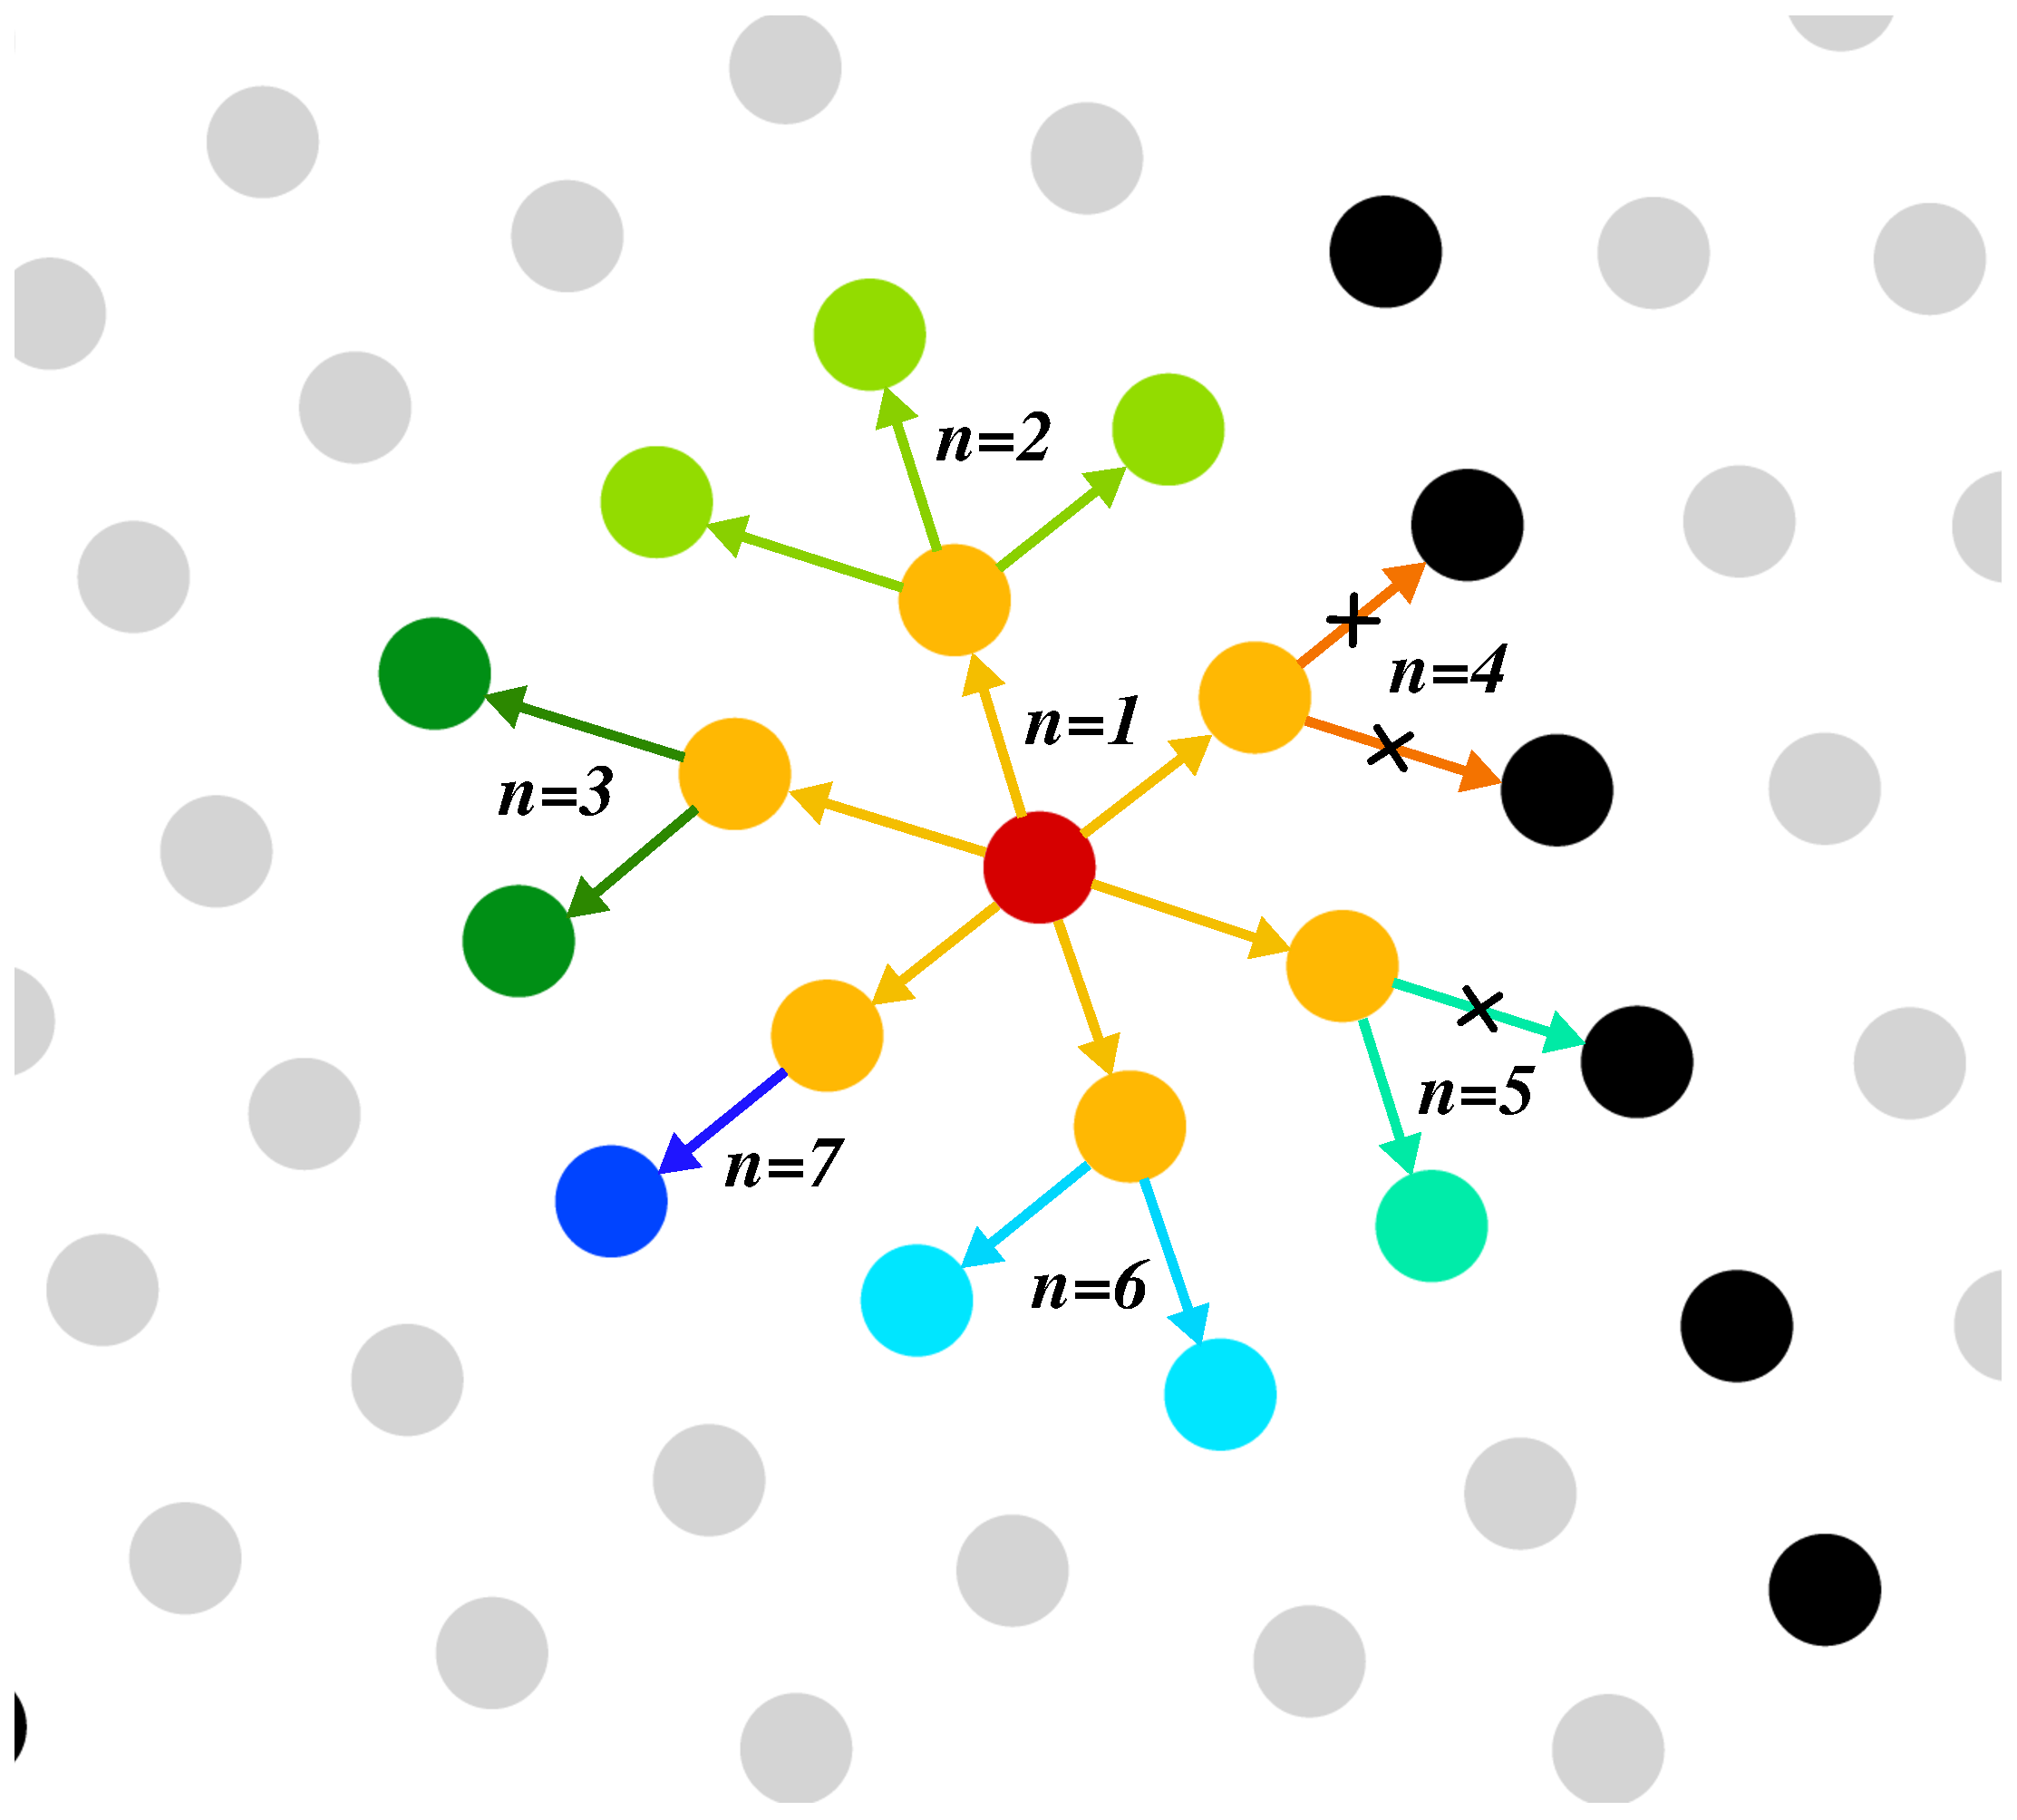
\includegraphics[width=60mm]{Pic/fig_A1.eps} 
	\end{center}
	\caption{Seven first iterations of the step by step twin identification algorithm; in light grey the atoms corresponding to a perfect FCC crystal structure (CNA = 1) and in black the atoms belonging to a stacking fault (CNA = 2). Colours are superimposed to display the growth of the detected twinned zone.}\label{fig_A1}
\end{figure}

\paragraph{Identification of twin boundaries}
Atoms in a TB are characterized by a CNA parameter equal to 2, corresponding to a compact hexagonal local structure. Thus they have not been identified in the previous step of the algorithm. Here again, a function ($ f^{tb} $) is created, which will return, for an atom $ i $ belonging to a TB, the ID of the twin considered. For example, if an atom $ i $ is in the boundary of the twin whose ID is 2 then $ f^{tb}_{i}=2 $. On the other hand, if the atom is not in a TB, the returned value will be zero ($ f^{tb}_{i}=0 $). Here only atoms whose CNA parameter is equal to 2 are scanned. These atoms can belong either to a stacking fault (ISF), generated by one Shockley dislocation, or to a TB. To differentiate between ISF and TB, it is sufficient to look if a twin has been identified in the close proximity of the scanned atom; if it is the case, the ID of the nearby twin will be assigned to it ($ f^{tb}_{i}=ID $). Thus, an atom whose CNA parameter is 2 is considered in a TB if it has at least two neighbour atoms $ j $ belonging to a twin ($ f^{twin}_{j}=ID $) and two others belonging to a non-twinned crystal ($ f^{twin}_{j}=0 $). 

\paragraph{Final check}
In some cases, a group of atoms may be erroneously identified as a twin by the algorithm. It is the case for example for atoms crossed by a full lattice dislocation: the local rotation induced by this dislocation is close to $ 19.47^{\circ} $ and after the passage of the dislocation these atoms are again in a perfect FCC environment. Therefore, this group of atoms has been identify as a twin by the algorithm but can not be considered as a ``real" twin and must be removed from the list. Such a group of atoms has no TB associated to it, so that the final check is to test if the twins identified by the algorithm have a TB associated with them, in which only case they are kept in the twin list.
\newline

\noindent\textbf{References}
\bibliographystyle{elsarticle-num}
\bibliography{Bib/test_bib}


\end{document}
\endinput


